A \textbf{fractal} is an object that displays self-similarity under magnification and can be constructed using a simple motif (an image repeated on ever-reduced scales).\\
A \textbf{fractal} is an object that has noninteger fractal dimension (See Section \ref{sec:fd}).
\subsection{The Cantor Set}
\begin{wrapfigure}{r}{0.3\linewidth}
	\centering
	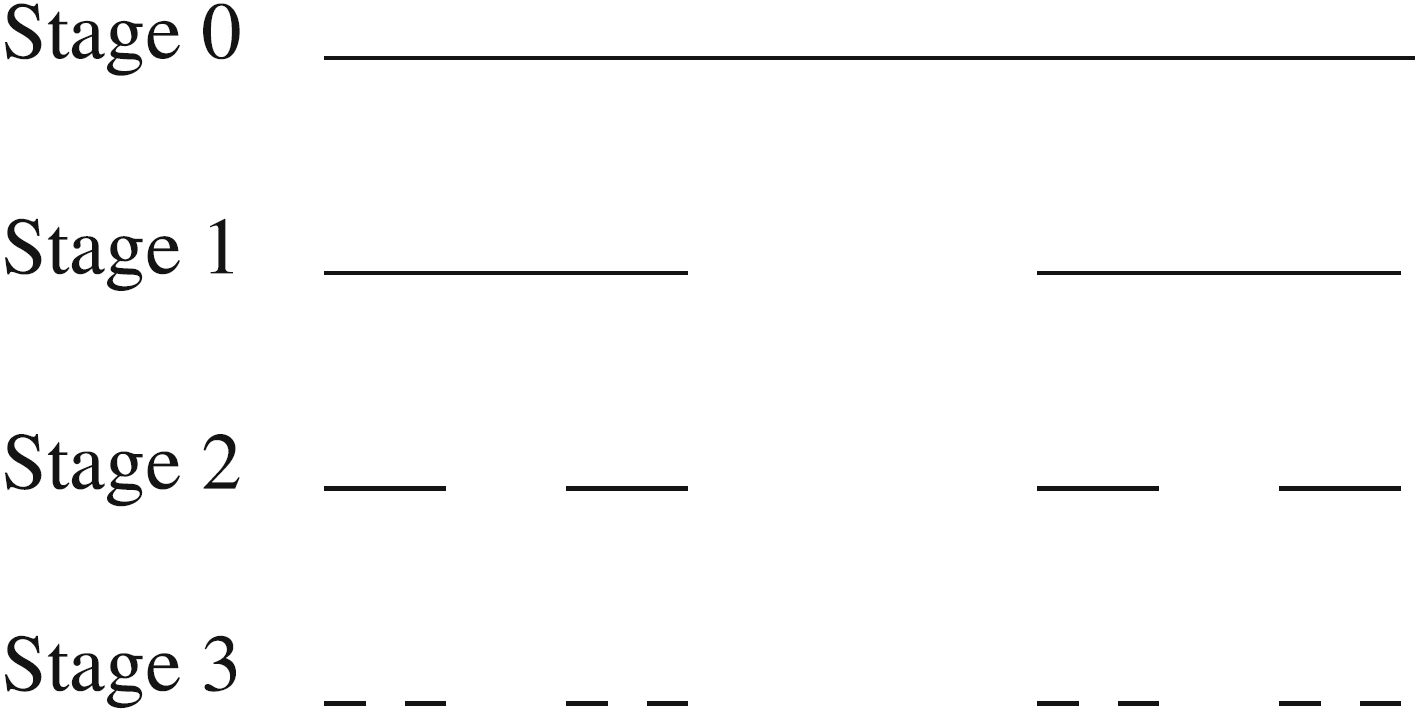
\includegraphics[width=\linewidth]{tcs.png}
	\caption{An early generation of the Cantor set.}
	\label{fig:tcs}
\end{wrapfigure}
It is constructed by removing the middle third of a line segment at each stage of construction.
Thus, at stage 0, there is one line segment of unit length.
At stage 1, the middle third is removed to leave two segments each of length $\frac{1}{3}$.
Continuing in this way, there will be $N=2^k$ segments each of length $l=3^{-k}$.\\
If this process is continued to infinity, then
\begin{equation}
	\lim_{k\rightarrow\infty}2^k=\infty\quad\text{and}\quad\lim_{k\rightarrow\infty}3^{-k}=0
\end{equation}
By using the\emph{ ternary number system}, it is possible to classify which points in the unit interval belong to the Cantor set and which do not.
The Cantor set can be identified by points whose ternary fractions consist of \emph{zeroes and twos} only.
\subsection{The Koch Curve}
It is constructed by replacing a unit line segment with a motif consisting of four line segments each of length $\dfrac{1}{3}$.
\begin{figure}[h!]
	\centering
	
\includegraphics[width=\linewidth]{tkc.png}
	\caption{Construction of the Koch curve up to stage 5.}
	\label{fig:tkc}
\end{figure}
At the $k^{th}$ stage there are $N=4^k$ line segments each of length $l=3^{-k}$.
\begin{equation}
	\lim_{k\rightarrow\infty}4^k=\infty\quad\text{and}\quad\lim_{k\rightarrow\infty}3^{-k}=0
\end{equation}
So the mathematical Koch curve consists of a curve that is infinitely long.
\subsection{Fractal Dimension}{\label{sec:fd}}
The concept of dimensions is quite intuitive as long as the dimension is a nonnegative integer and smaller or equal to three.
For simple geometrical objects like fixed points, limit cycles or tori the dimension is obvious, they are zero-, one- and two dimensional, respectively.\\
But what is the dimension of lorenz attractor? Its trajectory stays within a finite volume, it is not closed (in which case it would be a limit cycle), it does not cover a surface entirely as the quasi-periodic systems, nor does it fill a volume.\\
There are several ways to generalize the idea.
\subsubsection{Hausdorff index}
A self-similar fractal has fractal dimension (or Hausdorff index) $D_f$ given by
\begin{equation}
	D_f=\frac{\ln N(l)}{-ln l}\quad\equiv\quad N(l)\propto(l)^{-D_f}
\end{equation}
where $l$ represents a scaling and $N(l)$ denotes the number of segments of length $l$. 
\subsubsection{Correlation dimension}
We randomly distribute points along an interval on a line and within a square as shown in Figure (\ref{fig:fdcd}).
\begin{figure}[h!]
	\centering
	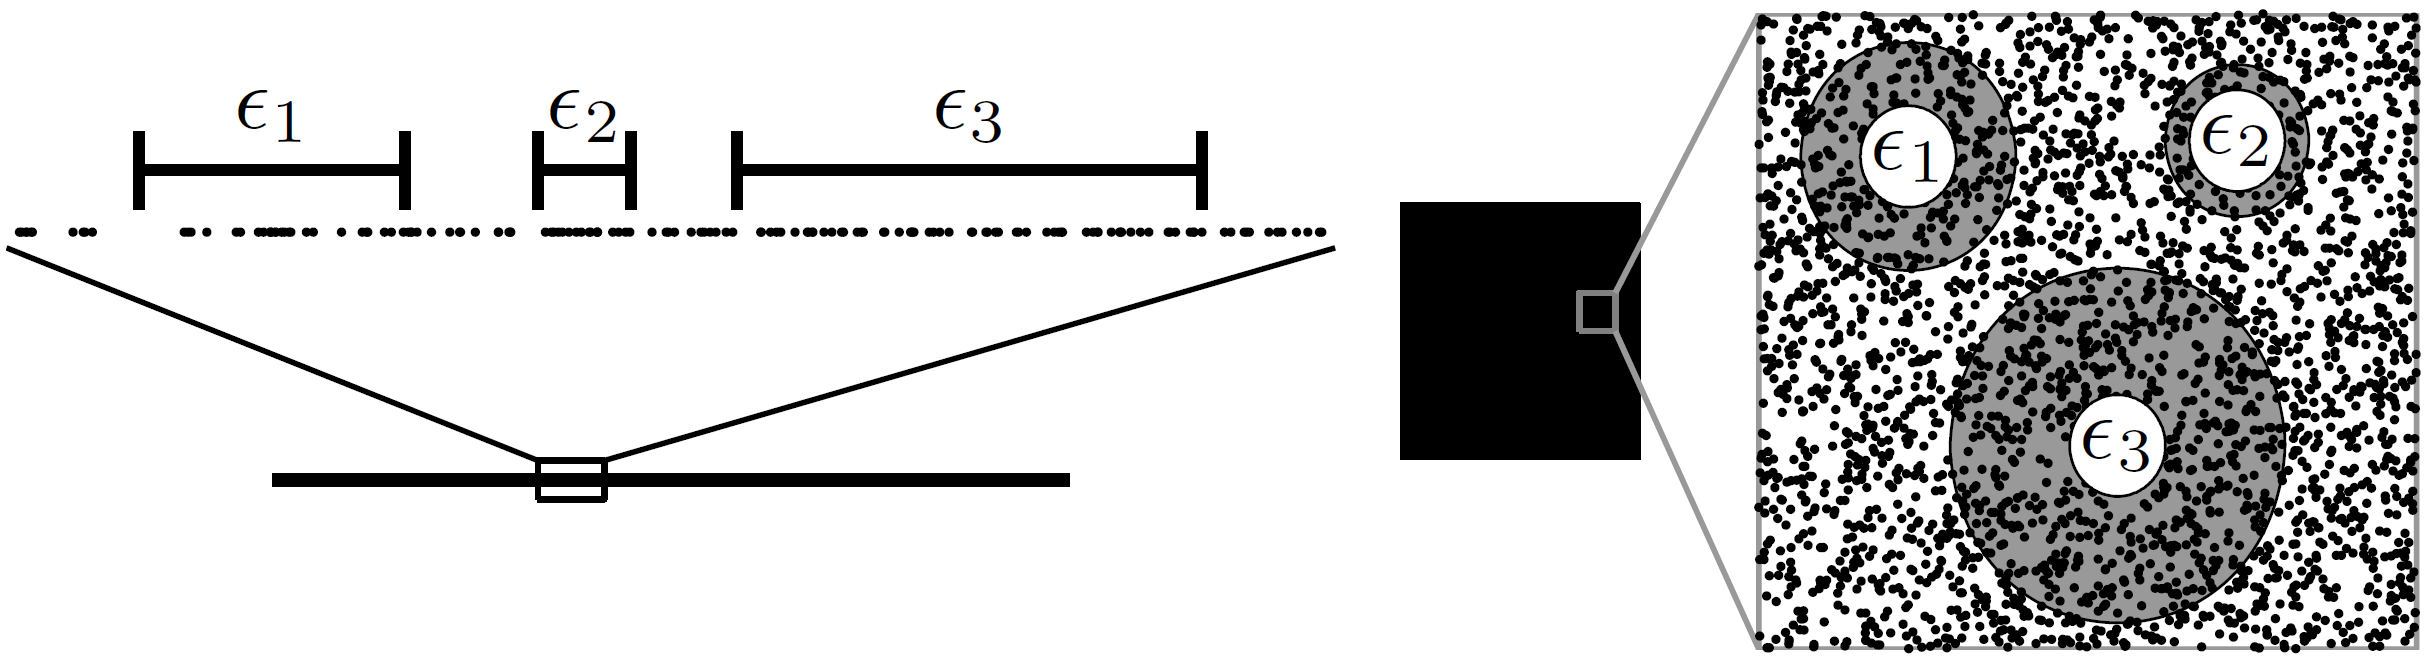
\includegraphics[width=0.4\linewidth]{fdcd.png}
	\caption{Determining the dimension of a line and a plane}
	\label{fig:fdcd}
\end{figure}
Now we pick one of these points and count how many other points are located within a distance $\epsilon$.
It is intuitively clear that for the one-dimensional line this number $N(\epsilon)$ will be proportional to $\epsilon$, for the two-dimensional square it will be proportional to $\epsilon^2$.
In general, the number of points within a radius $\epsilon$ from a given point $\mathbf{x}$ is proportional to $\epsilon^d$ where $d$ is a generalized dimension, the so-called pointwise dimension of that point.
The correlation dimension for an attractor is found by calculating and averaging $N(\epsilon)$ for all points on the attractor and plotting $\log N(\epsilon)$ as a function of $\log\epsilon$.
\begin{equation}
	N(\epsilon)\sim\epsilon^d\quad\rightarrow\quad N(\epsilon)=c\epsilon^d\quad\rightarrow\quad\log N(\epsilon)=d\log\epsilon+\log c
\end{equation}
\subsubsection{Generalised Fractal Dimensions}
The generalized (box-counting) fractal dimensions $D_q$, where $q\in\mathbb{R}$, are defined by
\begin{equation}
	D_q=\lim_{l\rightarrow0}\frac{1}{1-q}\frac{\ln\sum\limits_{i=1}^Np_i^q(l)}{-\ln l}\quad\text{where}\quad p_i(l)=\frac{N_i(l)}{N}
\end{equation}
Where the index $i$ labels the individual boxes of size $l$ and $p_i(l)$ denotes the relative weight of the $i^{th}$ box or the probability of the object lying in the box.
$N_i(l)$ is the weight of the $i^{th}$ box and $N$ is the total weight of the object.
\begin{equation}
	D_0=D_f=\lim_{l\rightarrow0}\frac{\ln N(l)}{-\ln l}\quad
	D_1=\lim_{l\rightarrow0}\frac{\sum\limits_{i=1}^Np_i\ln(p_i)}{-\ln l}
\end{equation}
The quantity $D_0$ is known as the \textbf{hausdorff dimension}.
The quantity $D_1$ is known as the \textbf{information dimension}.
The quantity $D_2$ is known as the \textbf{correlation dimension} and indicates the correlation between pairs of points in each box.
The generalized dimensions $D_3,D_4,\ldots$ are associated with correlations between triples, quadruples, etc., of points in each box.
\subsection{Iterated Function Systems}
An iterated function system consists of several affine transformations which are applied in a random fashion, a procedure sometimes called the \textbf{chaos game}.\\
Affine transformations are linear transformations where a vector is rotated, scaled and shifted.
\begin{equation}
	\begin{pmatrix}
		x_{n+1}\\y_{n+1}
	\end{pmatrix}=
	\begin{pmatrix}
		a&b\\c&d
	\end{pmatrix}
	\begin{pmatrix}
		x_n\\y_n
	\end{pmatrix}+
	\begin{pmatrix}
		e\\f
	\end{pmatrix}\quad\equiv\quad
	\begin{pmatrix}
		x_{n+1}\\y_{n+1}\\1
	\end{pmatrix}=
	\begin{pmatrix}
		a&b&e\\c&d&f\\0&0&1
	\end{pmatrix}
	\begin{pmatrix}
		x_n\\y_n\\1
	\end{pmatrix}
\end{equation}
The rules of the chaos game can be generalized as follows:
\begin{itemize}
	\item Create two or more affine linear transformations.
	\item Assign probabilities to each of the transformations.
	\item Start with an initial point.
	\item Select a random transformation to get a second point.
	\item Repeat the process.
\end{itemize}
\begin{figure}[h!]
	\centering
	\begin{subfigure}{0.45\linewidth}
		\centering
		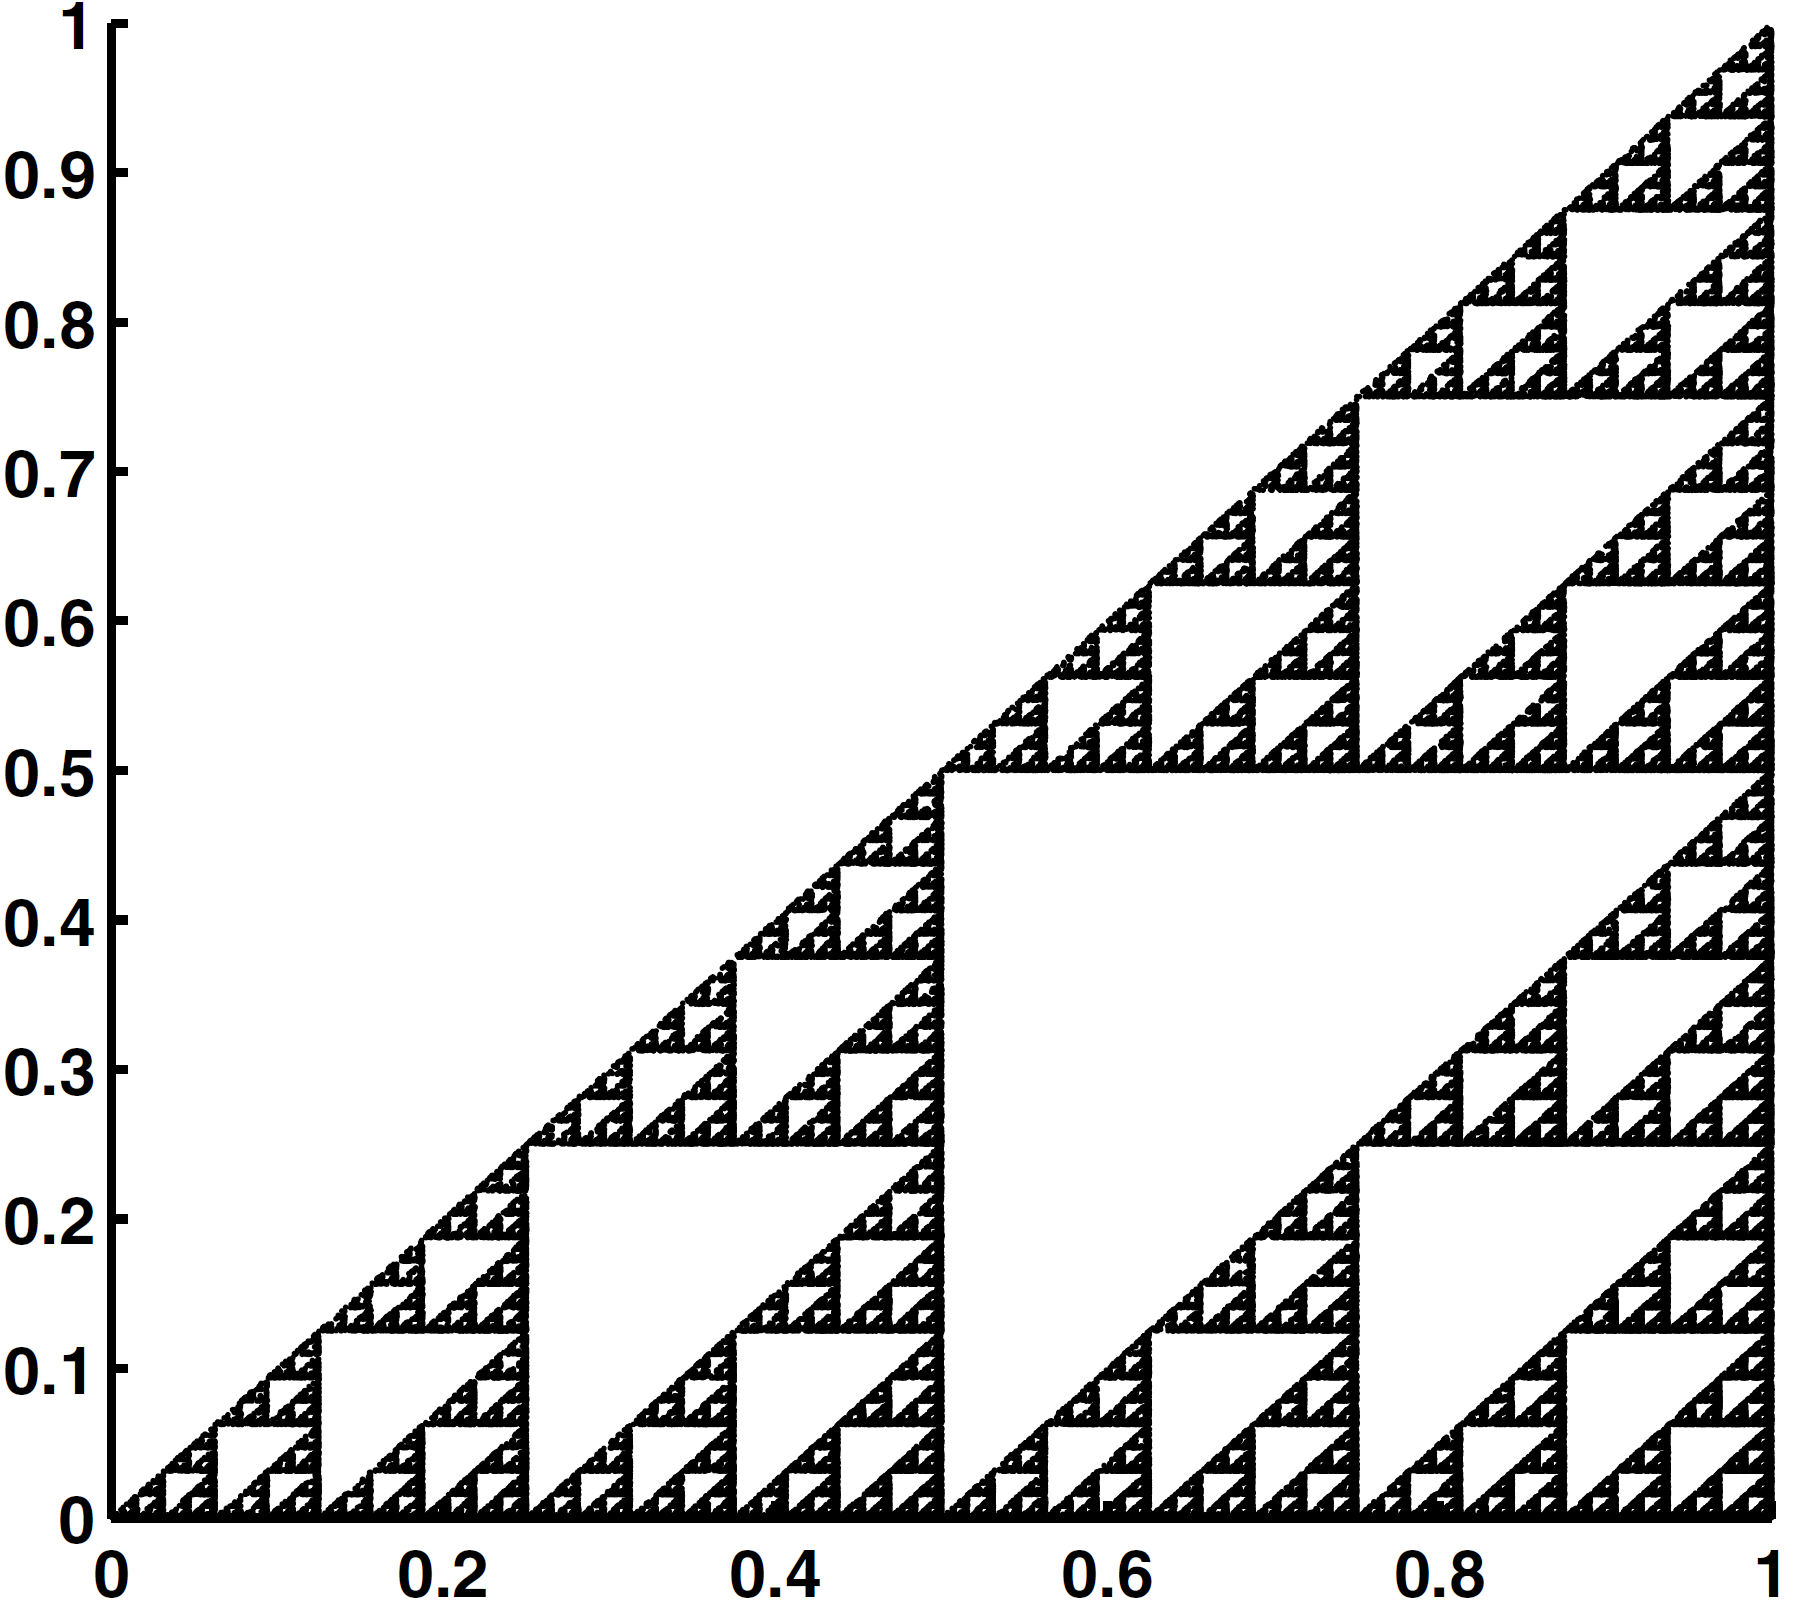
\includegraphics[width=\linewidth]{ifssg.png}
		\caption{The Sierpinsky triangle or gasket}
		\label{fig:ifssg}
	\end{subfigure}
	\vline
	\begin{subfigure}{0.4\linewidth}
		\centering
		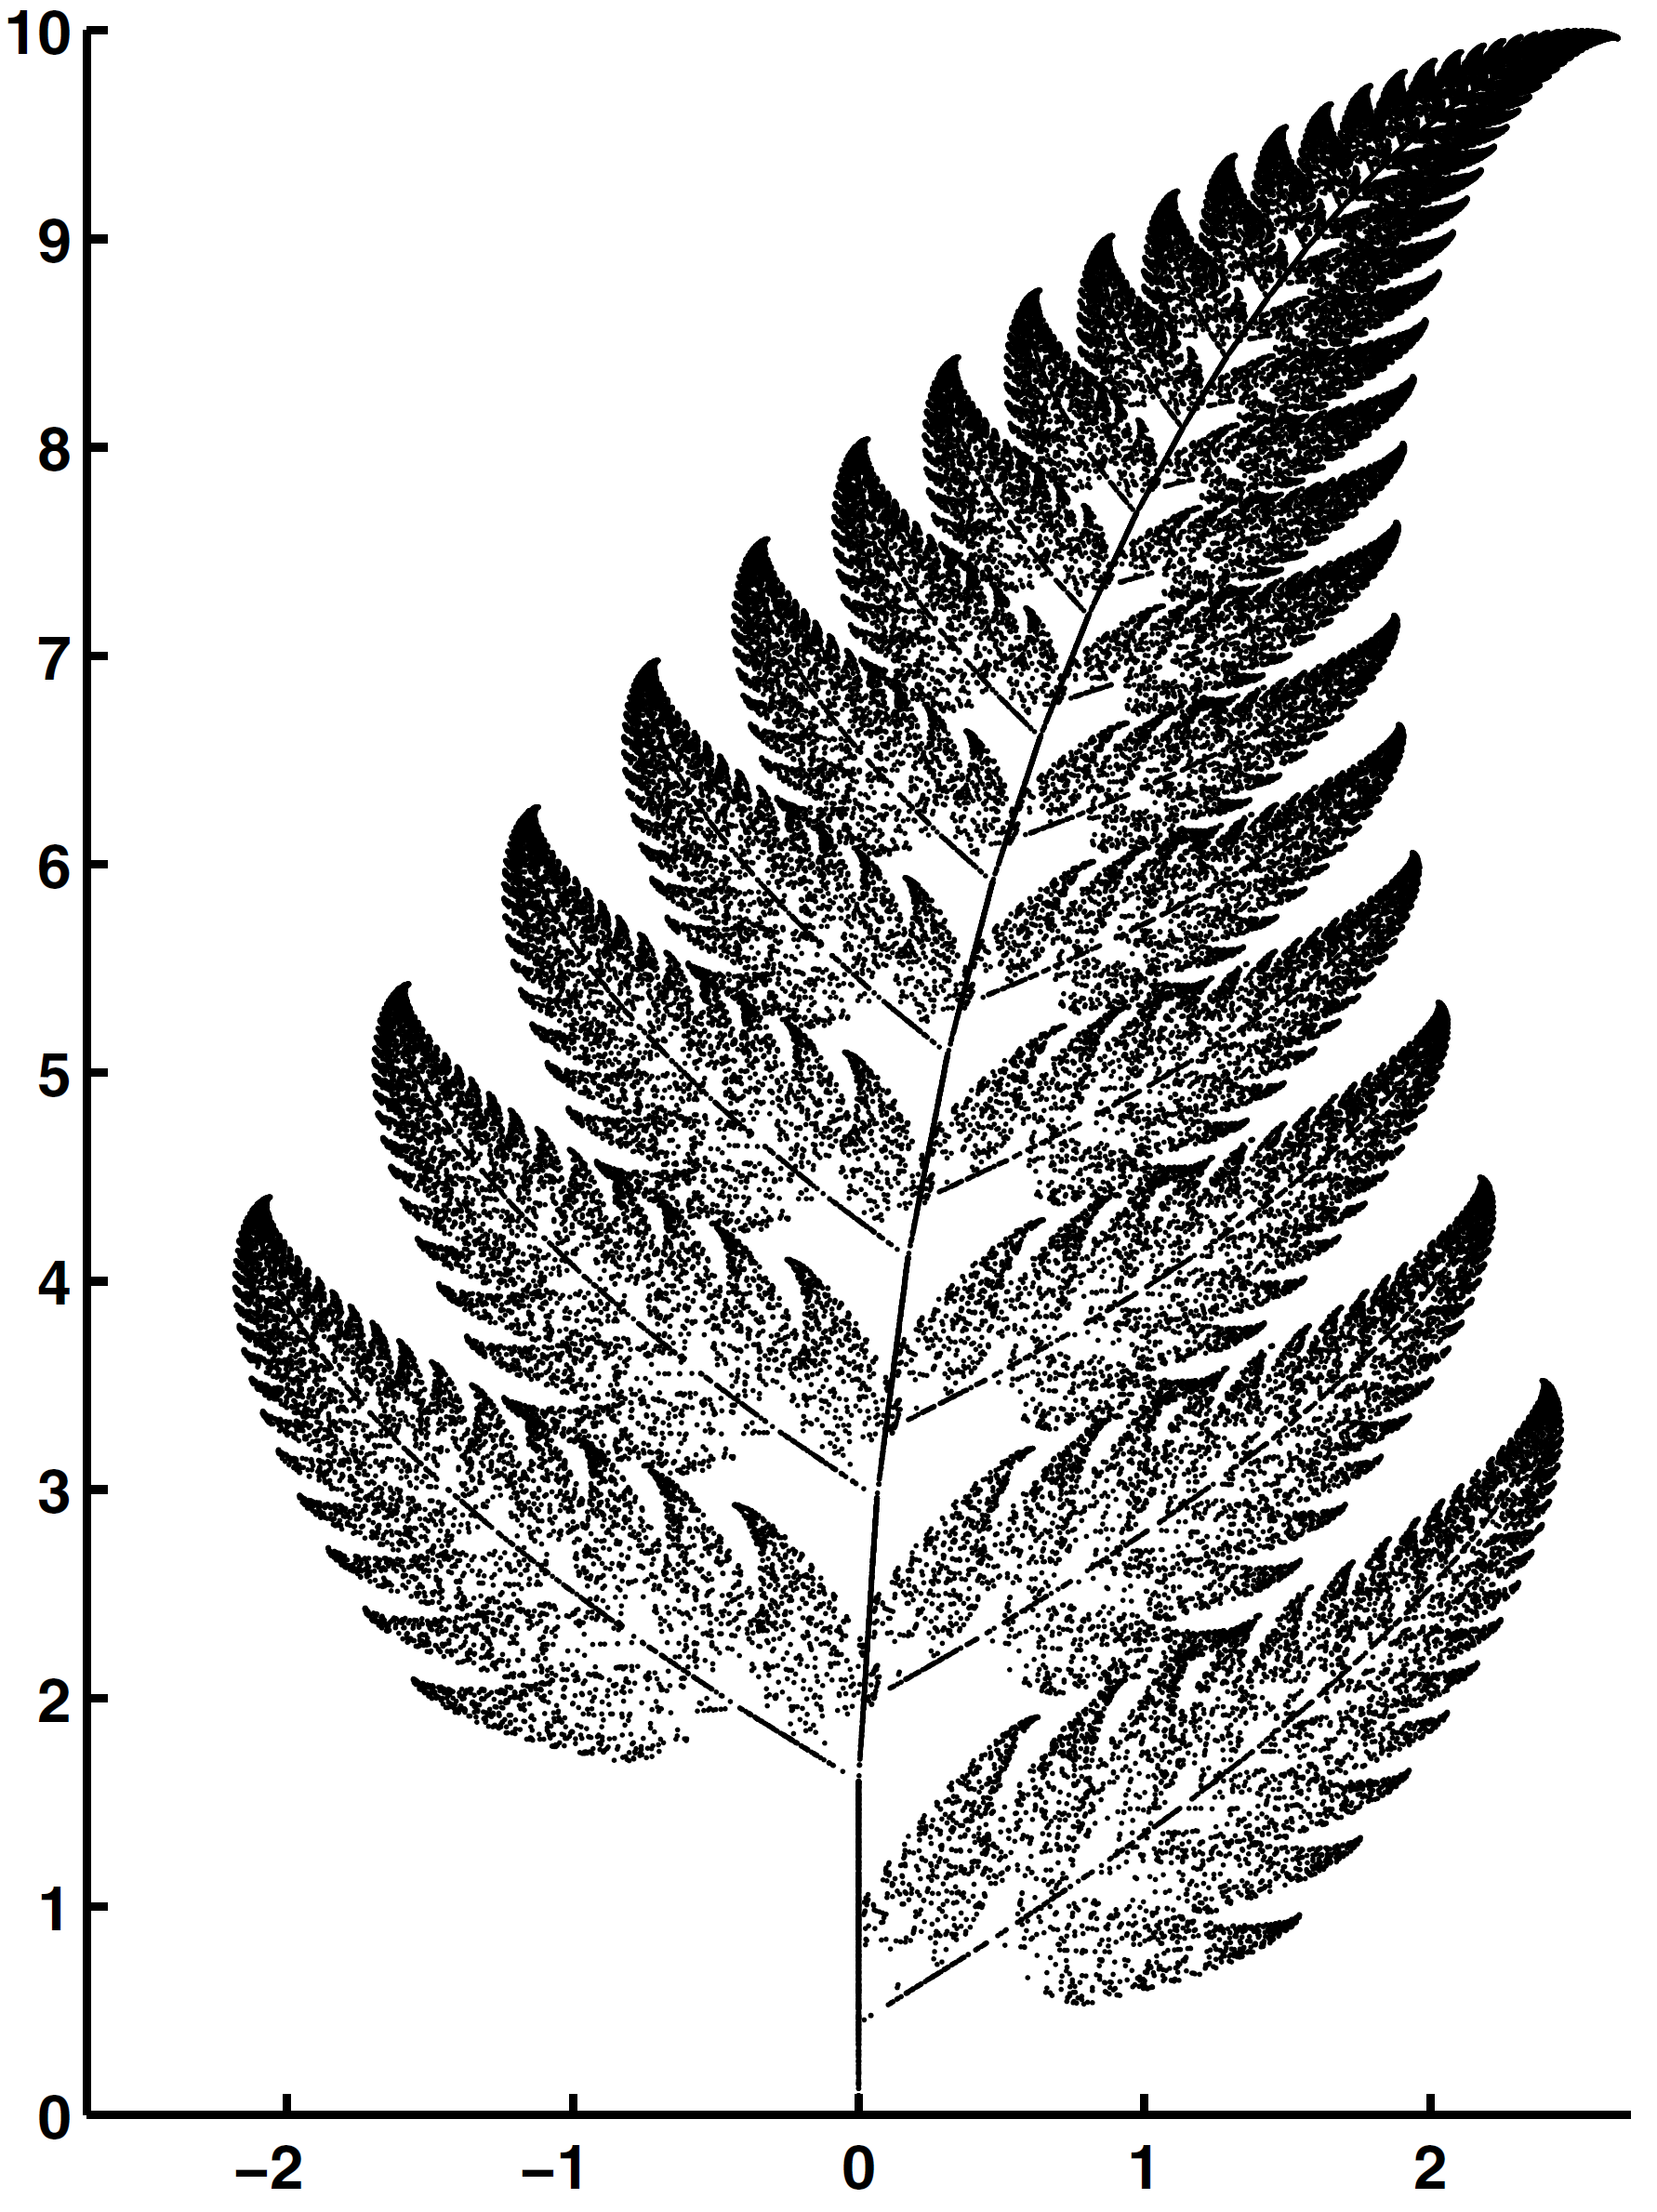
\includegraphics[width=\linewidth]{ifsbf.png}
		\caption{Barnsley’s fractal fern}
		\label{fig:ifsbf}
	\end{subfigure}
	\caption{}
\end{figure}
\begin{figure}[h!]
	\centering
	\begin{subfigure}{0.35\linewidth}
		\centering
		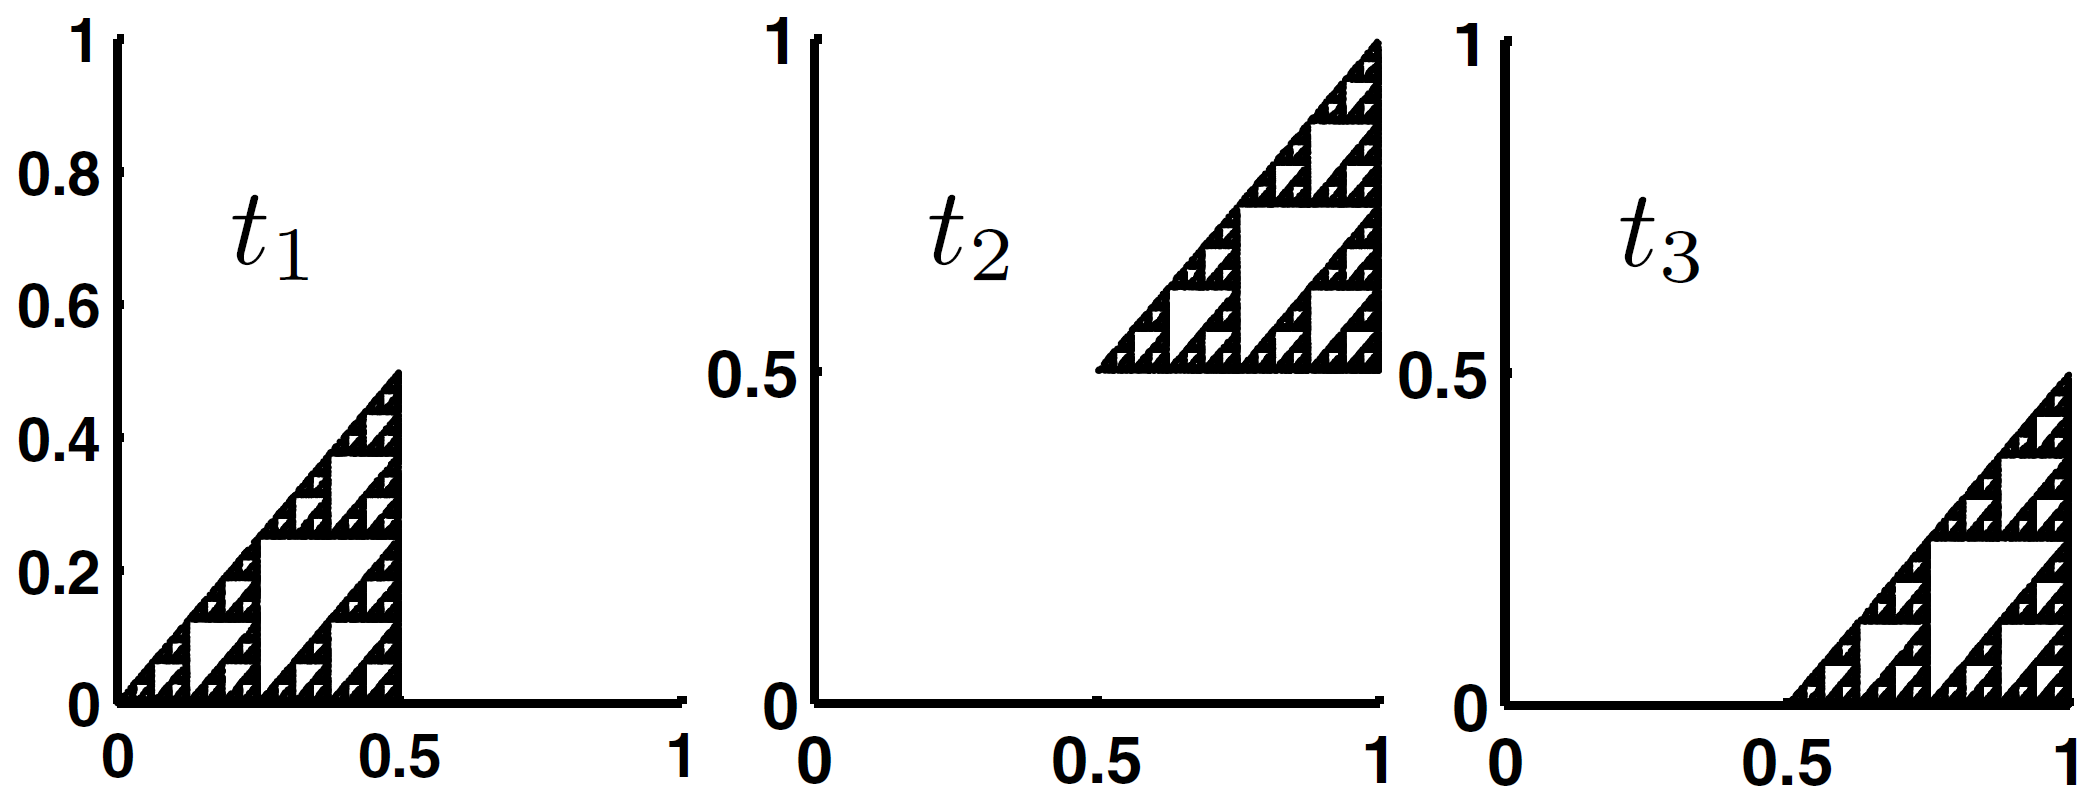
\includegraphics[width=\linewidth]{ifssgat.png}
		\caption{The regions that get covered when the transformations $t_1-t_3$ are applied.}
		\label{fig:ifssgat}
	\end{subfigure}
	\vline
	\begin{subfigure}{0.45\linewidth}
		\centering
		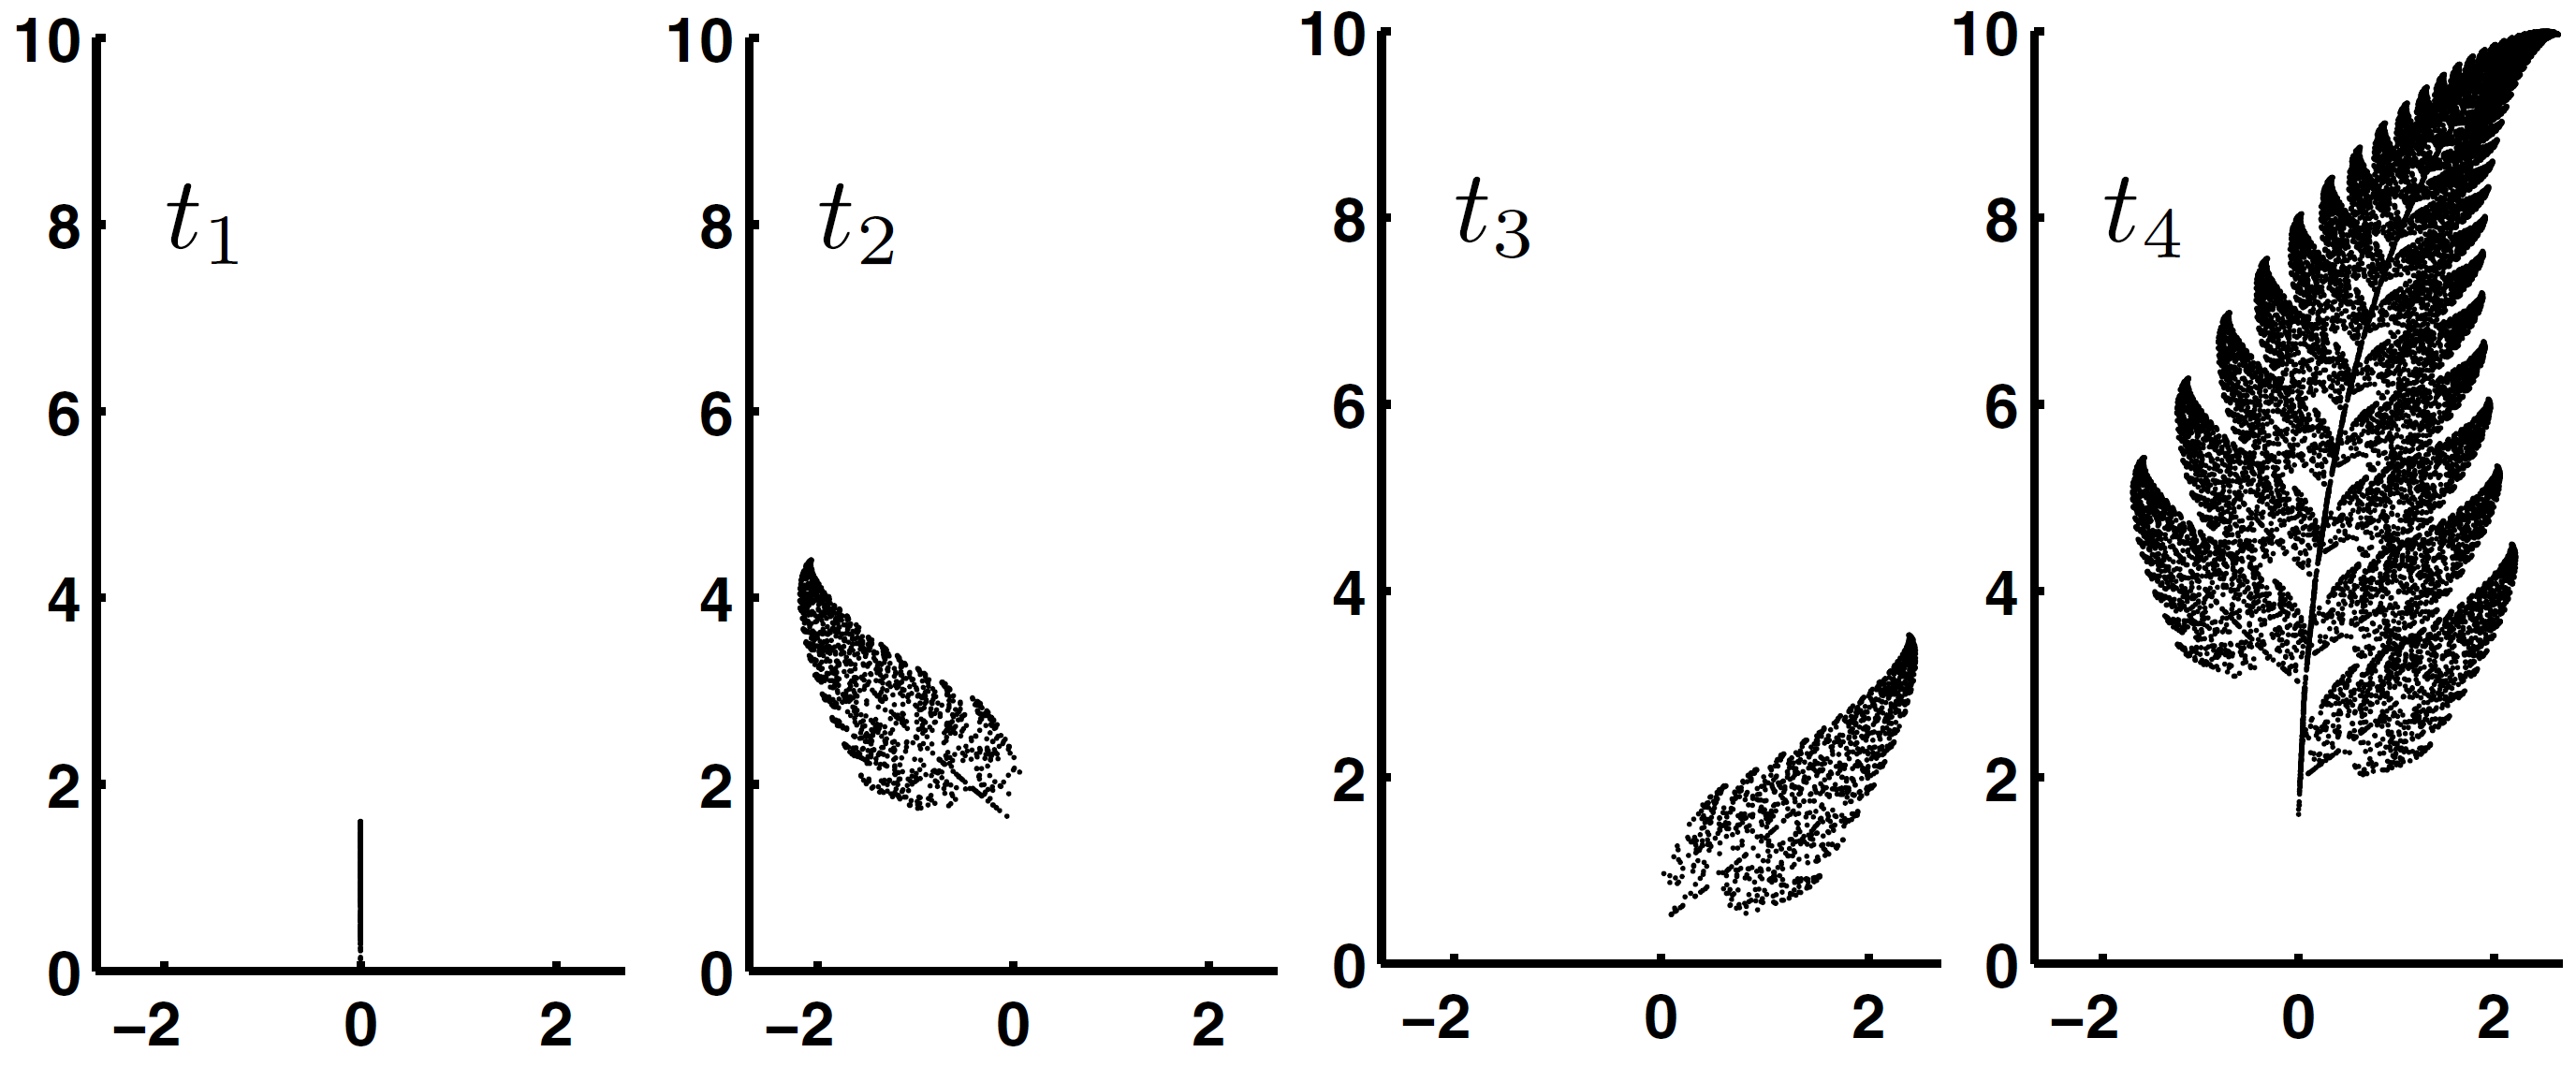
\includegraphics[width=\linewidth]{ifsbfat.png}
		\caption{The regions that get covered when the transformations $t_1-t_4$ are applied.}
		\label{fig:ifsbfat}
	\end{subfigure}
	\caption{}
\end{figure}
\subsubsection{Sierpinsky gasket}
This structure is constructed geometrically by starting with a solid black triangle and removing the large white triangle in the middle which leaves three black triangles after the first iteration step.
Then this procedure is applied to each of these triangles leading to nine smaller ones and so on.
{\renewcommand{\arraystretch}{1.2}
\begin{table}[h!]
	\centering
	\caption{Parameters for Iterated Function Systems}
	\label{tab:ifs}
	\subfloat[Sierpinski gasket]{
	\begin{tabular}{c c c c c c c c}
		&a&b&c&d&e&f&p\\
		\hline
		$t_1$&0.5&0&0&0.5&0&0&1/3\\
		$t_2$&0.5&0&0&0.5&0.5&0.5&1/3\\
		$t_3$&0.5&0&0&0.5&0.5&0&1/3\\
	\end{tabular}
	}
	\quad\vline\quad
	\subfloat[Barnsley’s fractal fern]{
	\begin{tabular}{c c c c c c c c}
		&a&b&c&d&e&f&p\\
		\hline
		$t_1$&0&0&0&0.16&0&0&0.01\\
		$t_2$&0.2&$-$0.26&0.23&0.22&0&1.6&0.07\\
		$t_3$&$-$0.15&0.28&0.26&0.24&0&0.44&0.07\\
		$t_4$&0.85&0.04&$-$0.04&0.85&0&1.6&0.85\\
	\end{tabular}
	}
\end{table}}
\\The parameters for the three transformations that are used to create the Sierpinski gasket by an iterated function system are shown in Table (\ref{tab:ifs}a).
There is an additional column listing a parameter $p$, which is the probability that this particular transformation is applied.
Figure (\ref{fig:ifssgat}) are three plots showing the points of Figure (\ref{fig:ifssg}) that arise after the transformations $t_1$, $t_2$ and $t_3$ are executed.
In the case of the Sierpinski gasket they fall into the three triangular regions that remain after the big triangle in the middle is removed.
\subsubsection{Barnsley’s Fern}
The Fractal Fern shown in Figure (\ref{fig:ifsbf}) together with smaller plots of the regions that are created by using only the points after a particular transformation has been applied.\\\\
The basic idea of \textbf{fractal compression of images} is that if pictures of natural scenes (like a fern) are encoded as pixels, a high resolution is necessary to preserve the complex structure, resulting in a huge amount of bits that have to be stored.
In contrast, for the fern for instance, only $4\cdot7=28$ numbers are needed and the image can be restored at any desired resolution.\\
The problem is that even though there were attempts to develop algorithms for finding the transformations and parameters for encoding a general image, the most impressive examples of fractal compression still need human intervention.
\subsection{Complex Iterative Maps}
\subsubsection{Julia Sets}
Consider a complex polynomial mapping of the form $z_{n+1}=f(z_n)$.
The points that lie on the boundary between points that orbit under $f$ and are bounded and those that orbit under $f$ and are unbounded are collectively referred to as the \textbf{Julia set}.\\
Consider the quadratic map
\begin{equation}
	z_{n+1}=f_c(z_n)=z_n^2+c\quad\text{where}\quad z_n,c\in\mathbb{C}
\end{equation}
The following are properties of a Julia set, say, $J$
\begin{itemize}
	\item The set $J$ is a \textbf{repellor}. 
	\item The set $J$ is \textbf{invariant}. 
	\item An orbit on $J$ is either \textbf{periodic} or \textbf{chaotic}. 
	\item All \textbf{unstable periodic} points are on $J$. 
	\item The set $J$ is either \textbf{wholly} \textbf{connected} or \textbf{wholly} \textbf{disconnected}. 
	\item The set $J$ nearly always has \textbf{fractal} structure.
\end{itemize}
\begin{figure}[h!]
	\centering
	
\includegraphics[width=\linewidth]{js.png}
	\caption{Julia sets for $c=0,-0.72i,-0.1-0.88i,-0.6+0.2i,-0.6+0.45i,0.37+0.37i,-0.25-0.7i$}
	\label{fig:js}
\end{figure}
\subsubsection{The Mandelbrot Set}
The Mandelbrot Set is the collection of $c$ values for which the \textbf{Julia sets are connected}.\\\\
There is an efficient way to determine the Mandelbrot Set as follows:\\
If the orbit of $z_0=0$ for $f(z)=z^2+c$ is \textbf{bounded}, then $c$ is in the Mandelbrot set.\\
If the orbit is \textbf{not} \textbf{bounded}, then $c$ is not in the Mandelbrot set.
\begin{figure}[h!]
	\centering
	\begin{subfigure}{0.45\linewidth}
		\centering
		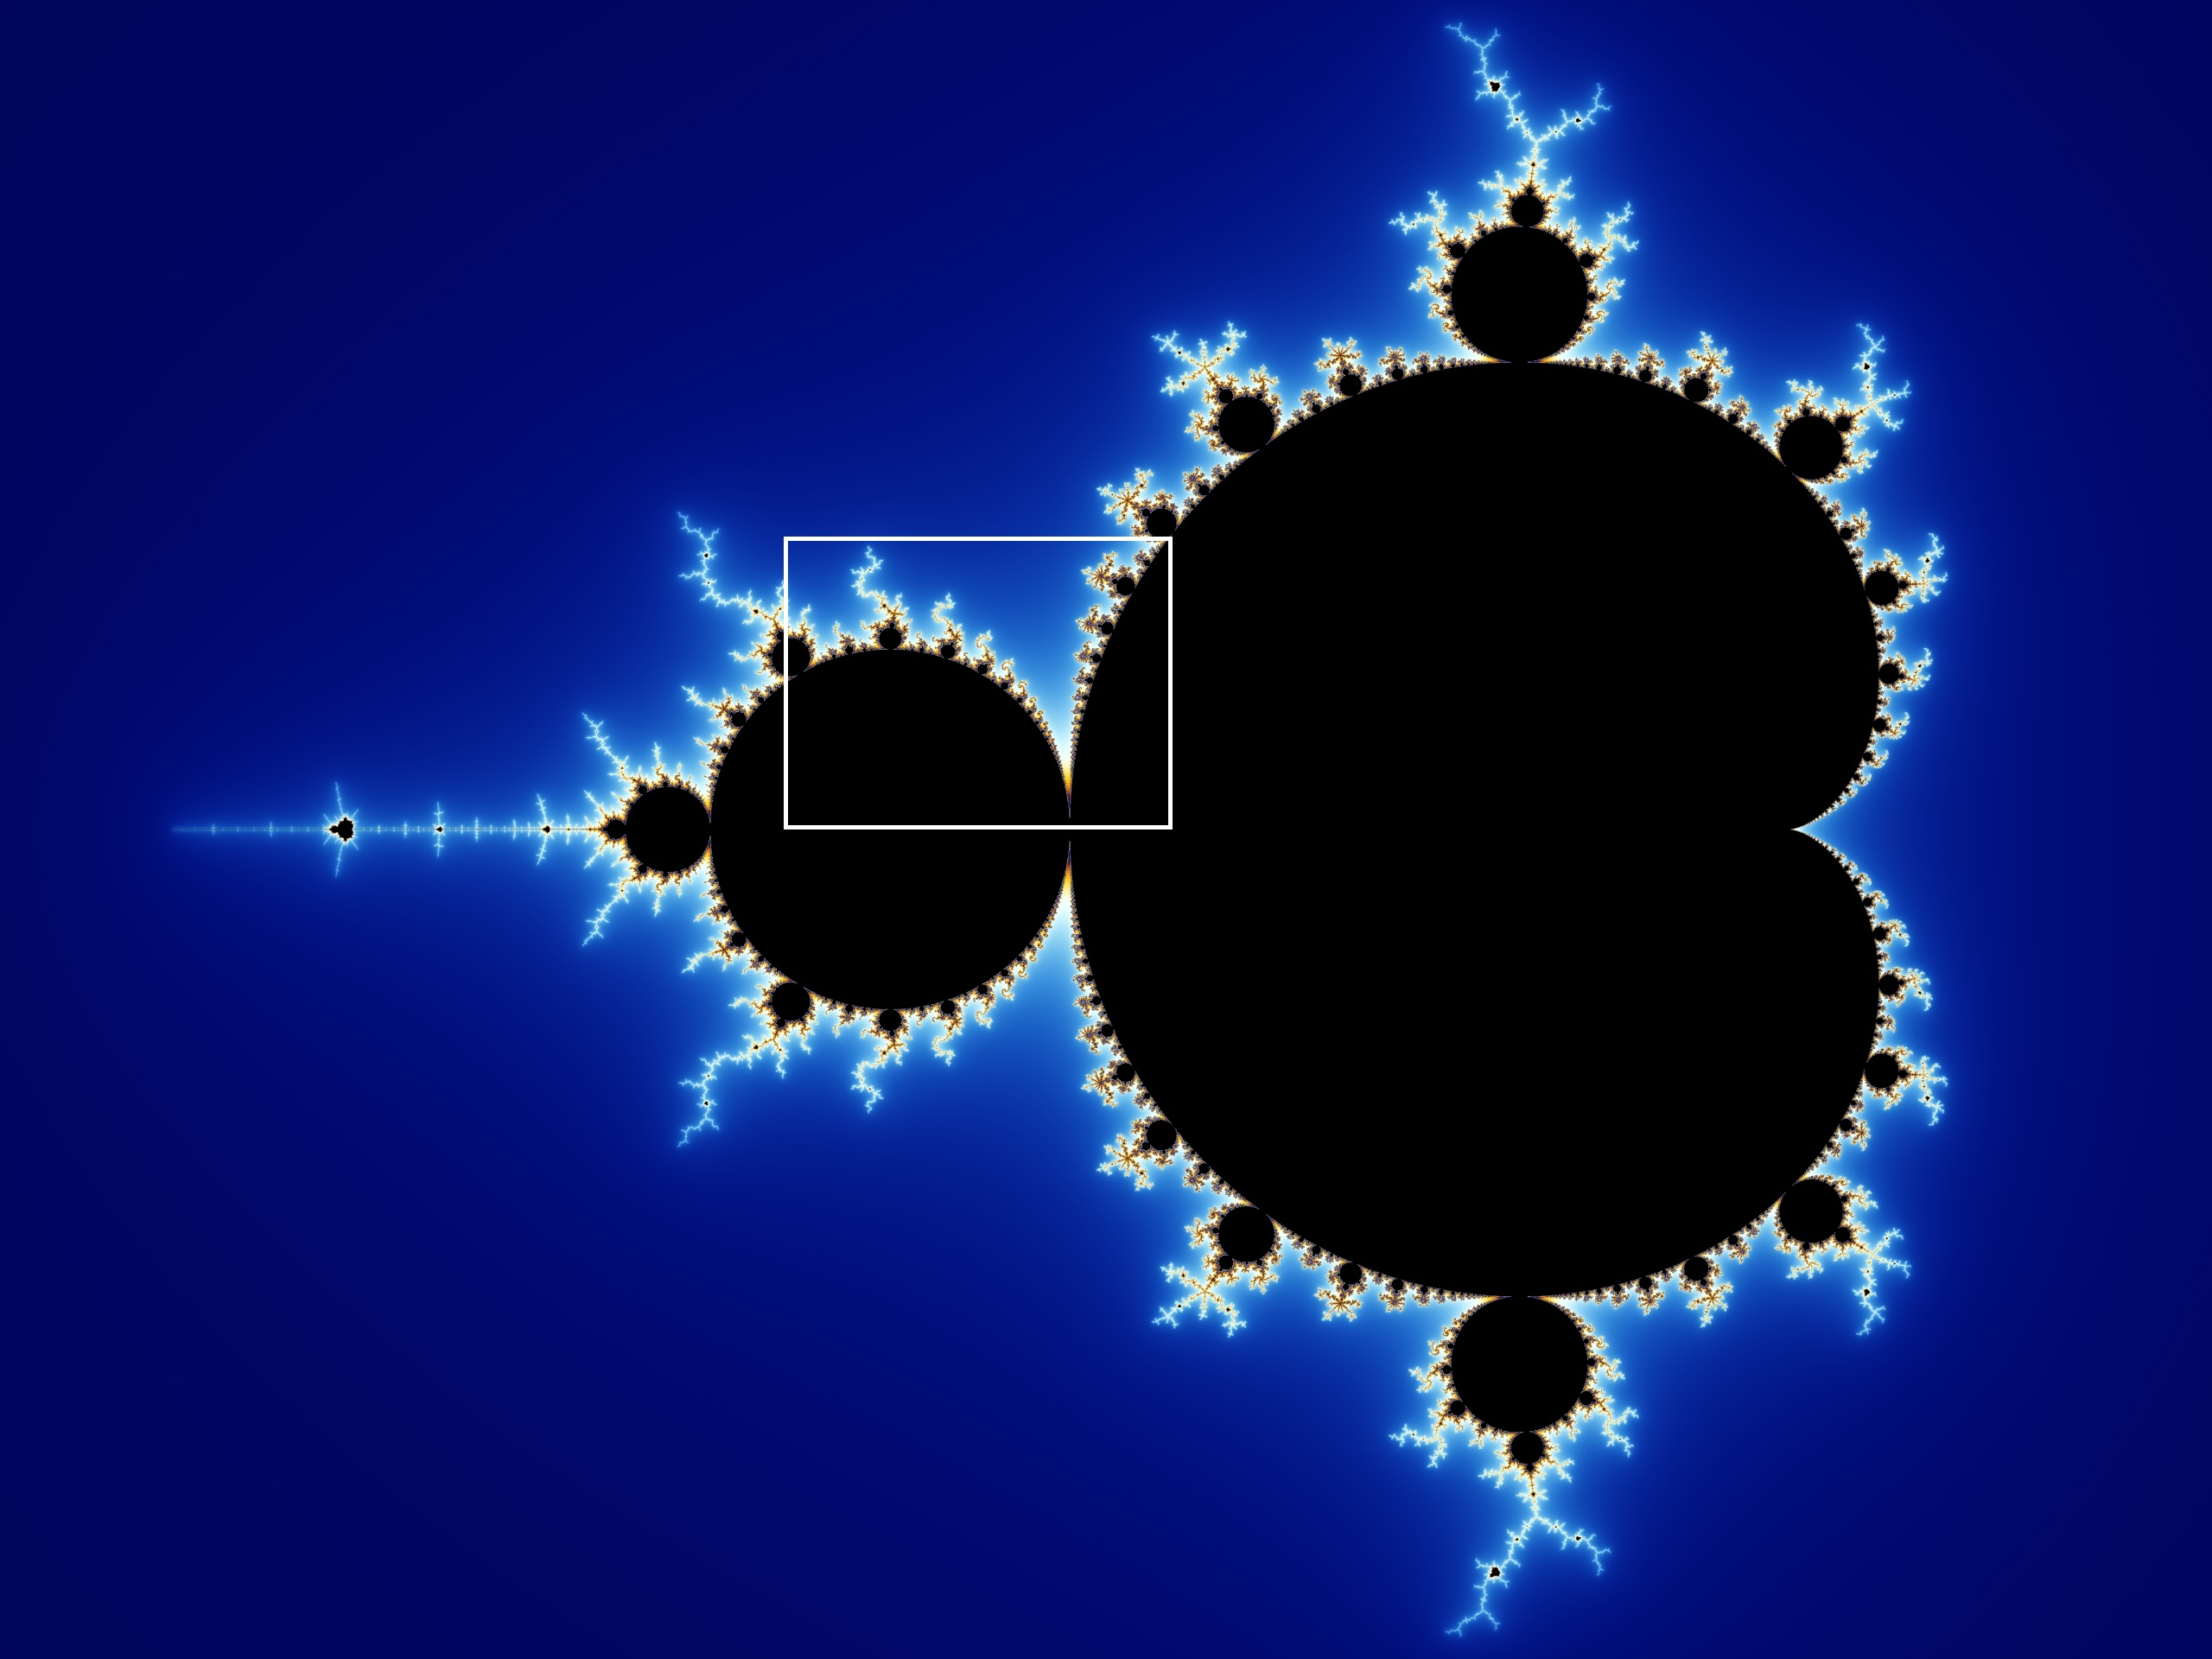
\includegraphics[width=\linewidth]{ms1.jpg}
		\caption{The Mandelbrot Set complete}
		\label{fig:ms1}
	\end{subfigure}
	\begin{subfigure}{0.45\linewidth}
		\centering
		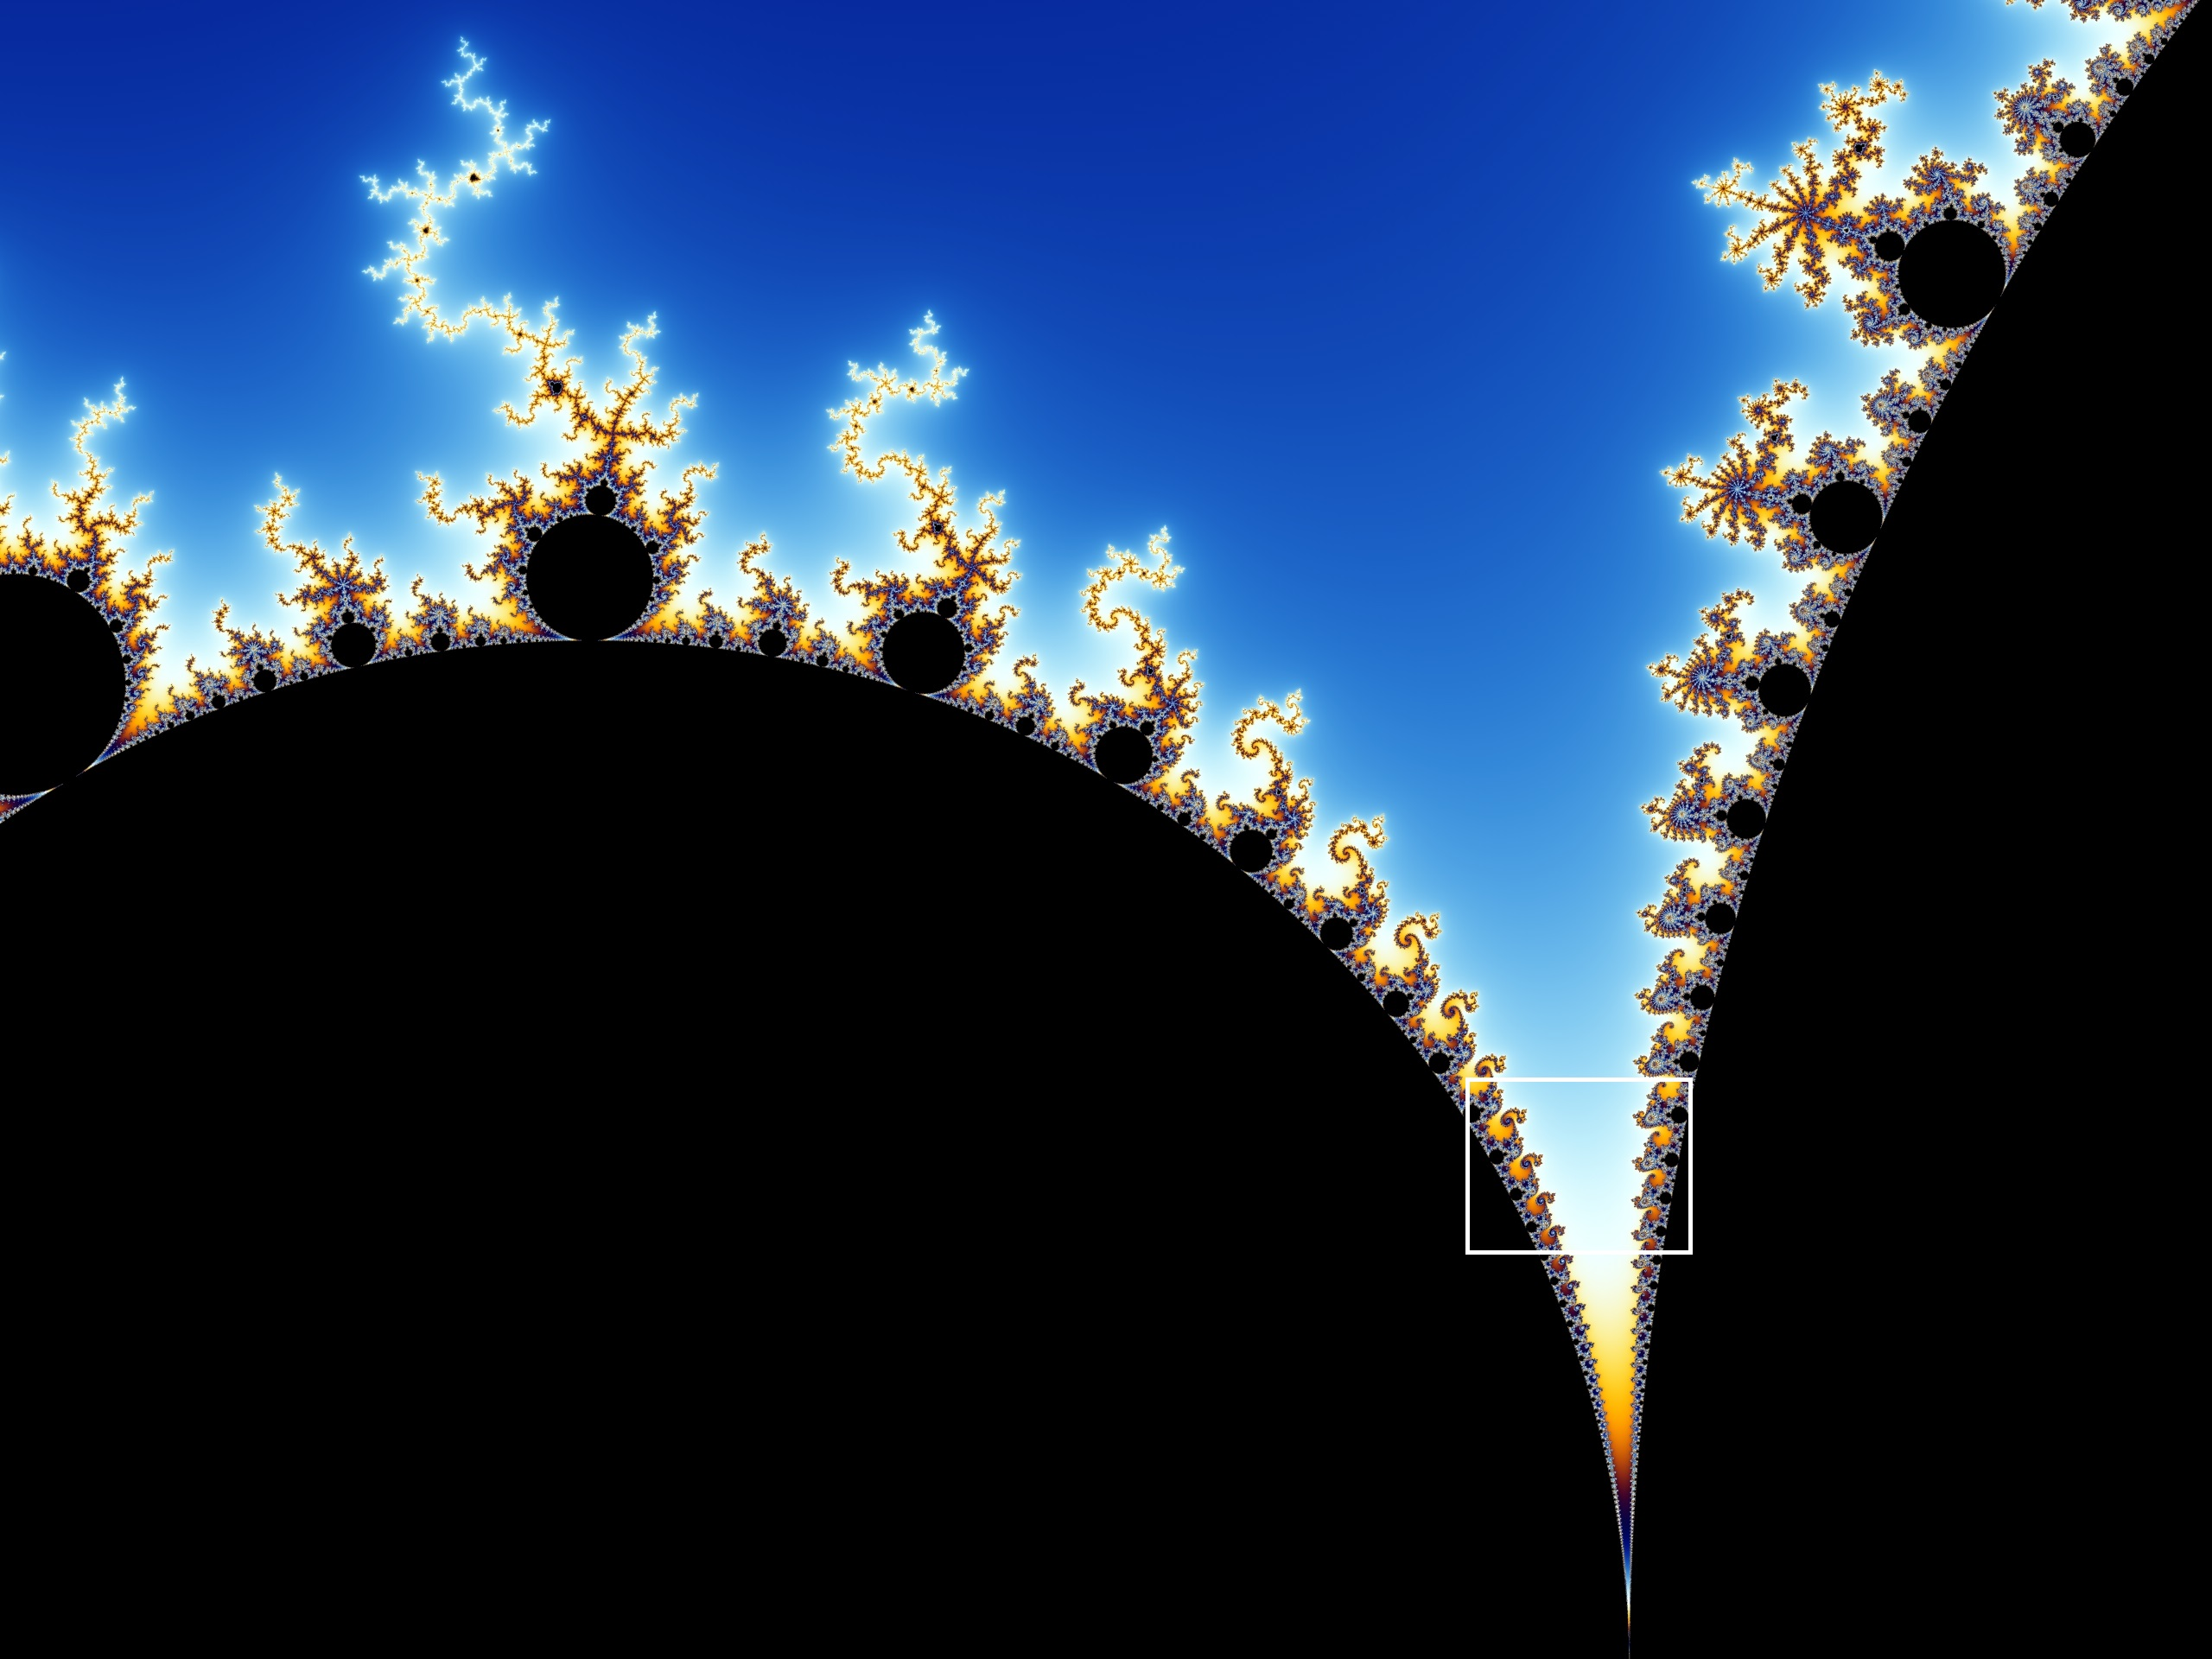
\includegraphics[width=\linewidth]{ms2.jpg}
		\caption{Seahorse Valley}
		\label{fig:ms2}
	\end{subfigure}
	\begin{subfigure}{0.45\linewidth}
		\centering
		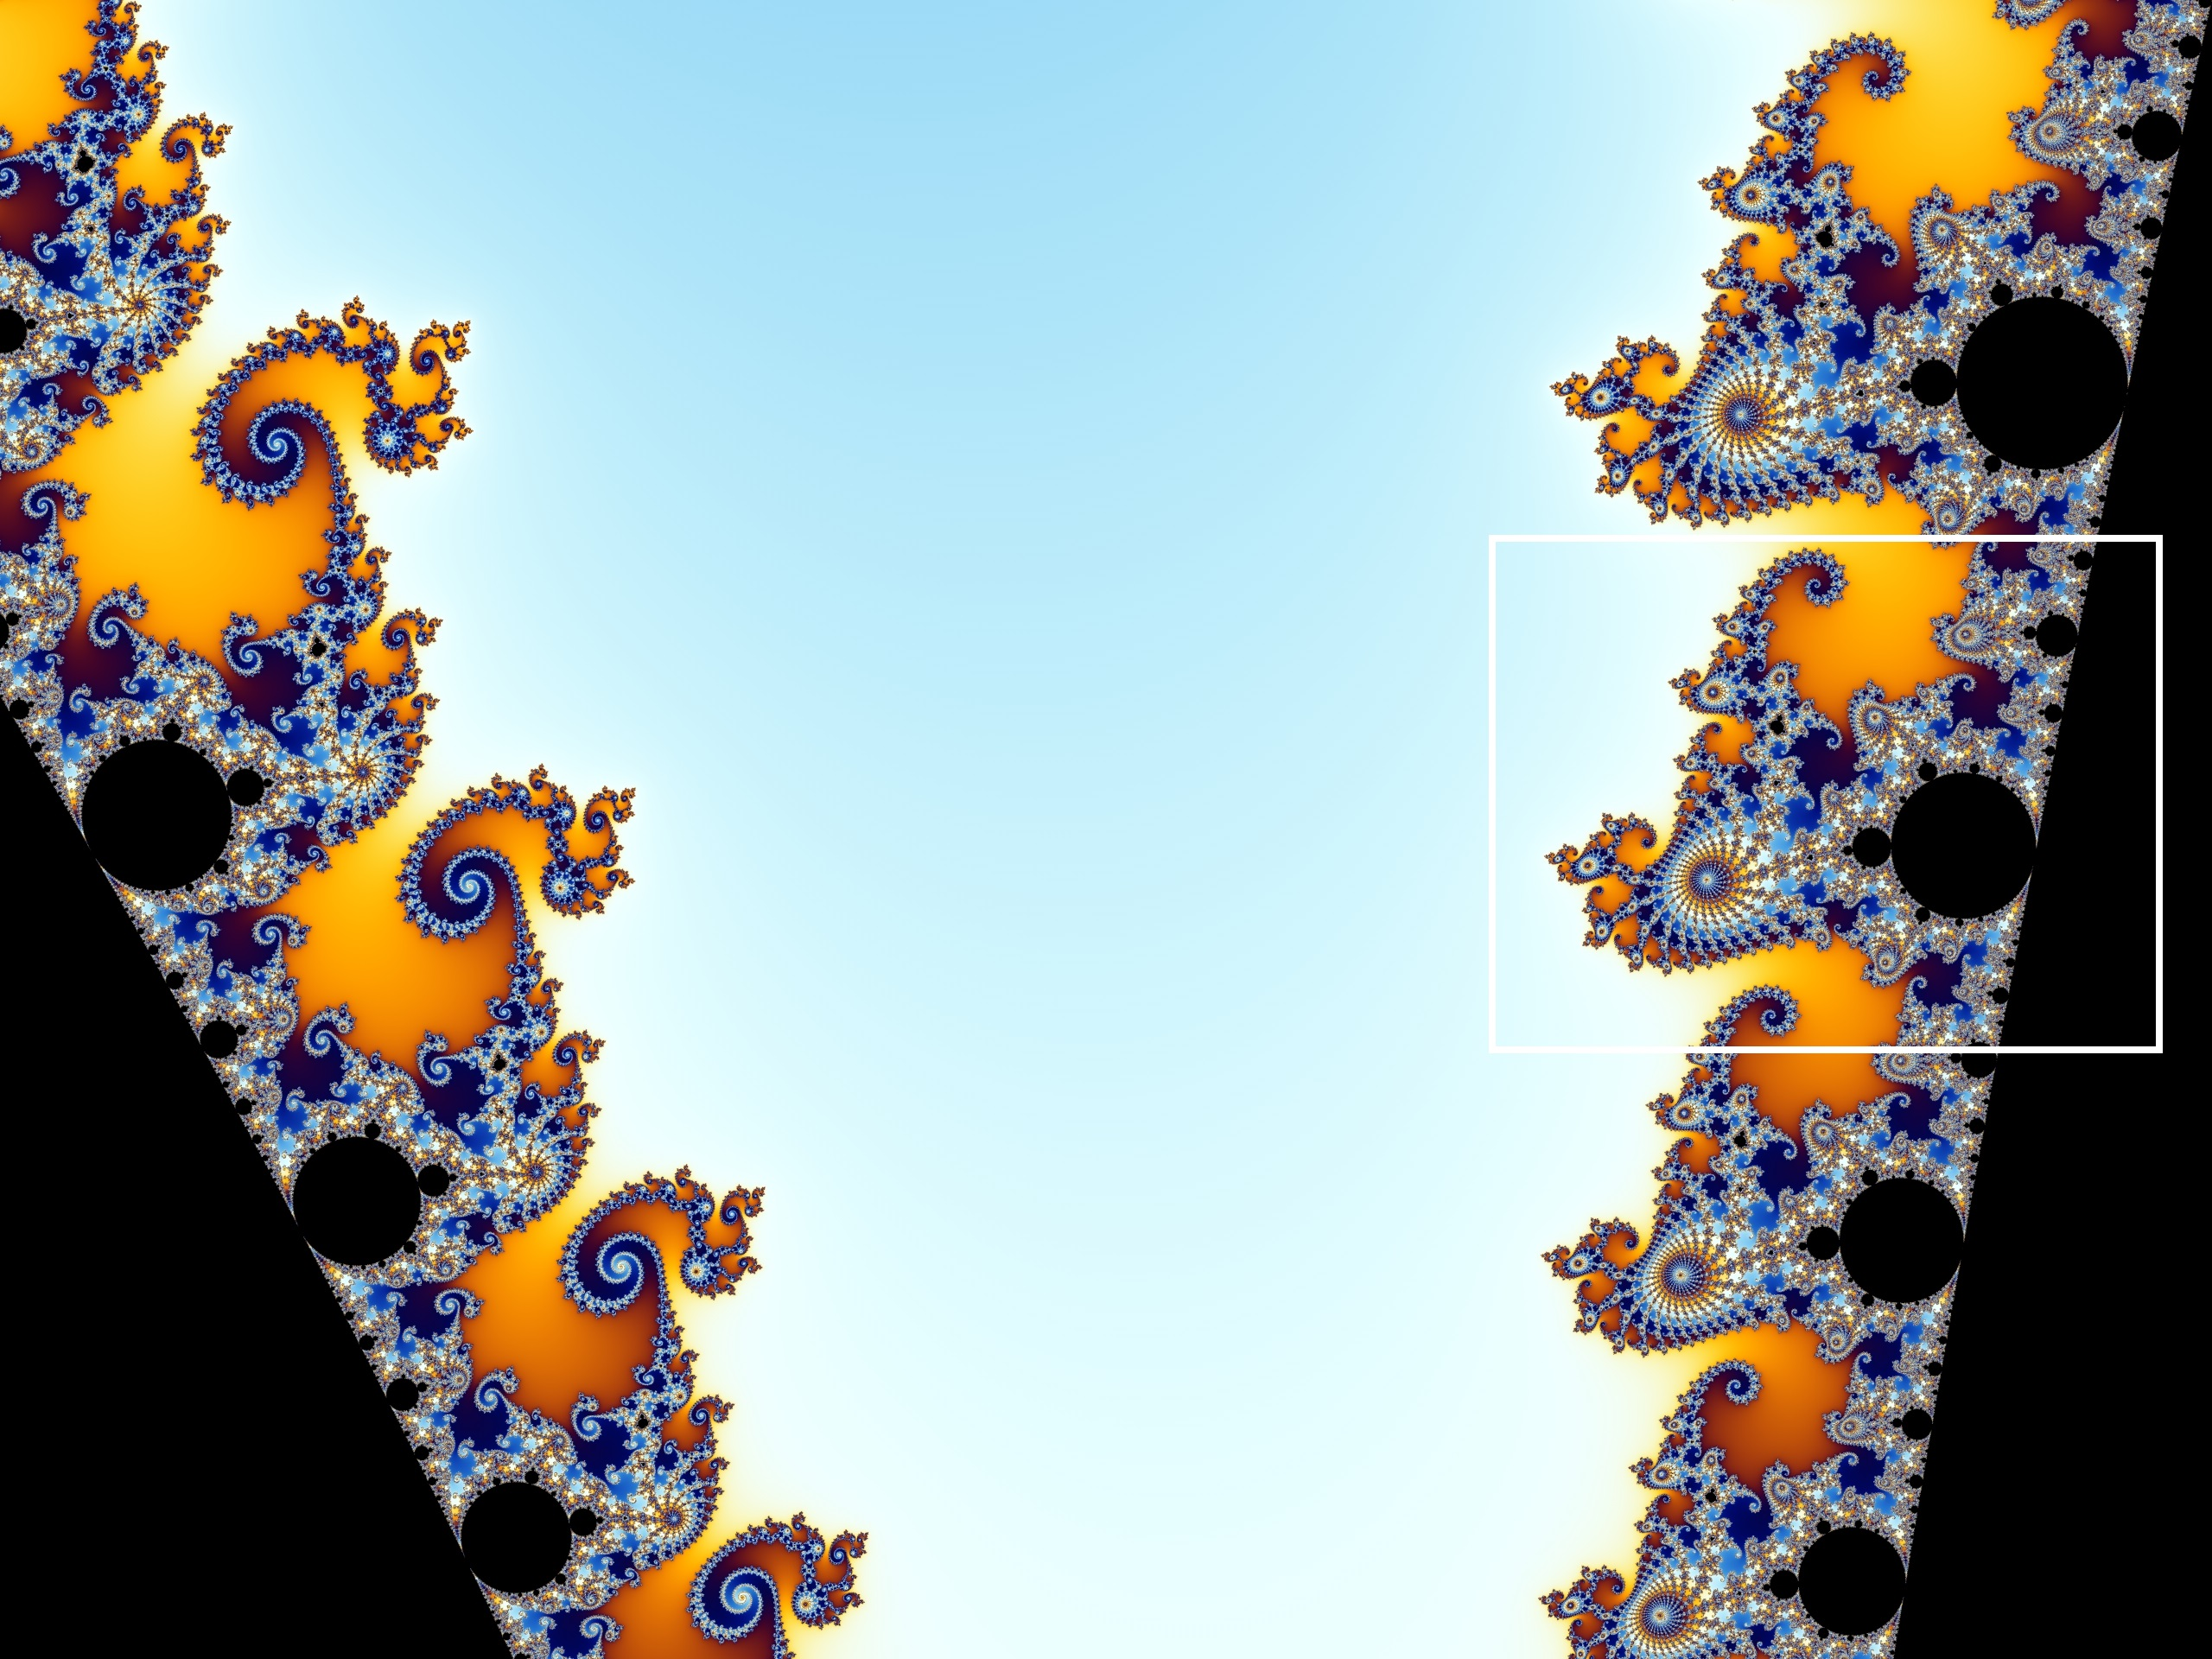
\includegraphics[width=\linewidth]{ms3.jpg}
		\caption{Seahorse Valley Zoom}
		\label{fig:ms3}
	\end{subfigure}
	\begin{subfigure}{0.45\linewidth}
		\centering
		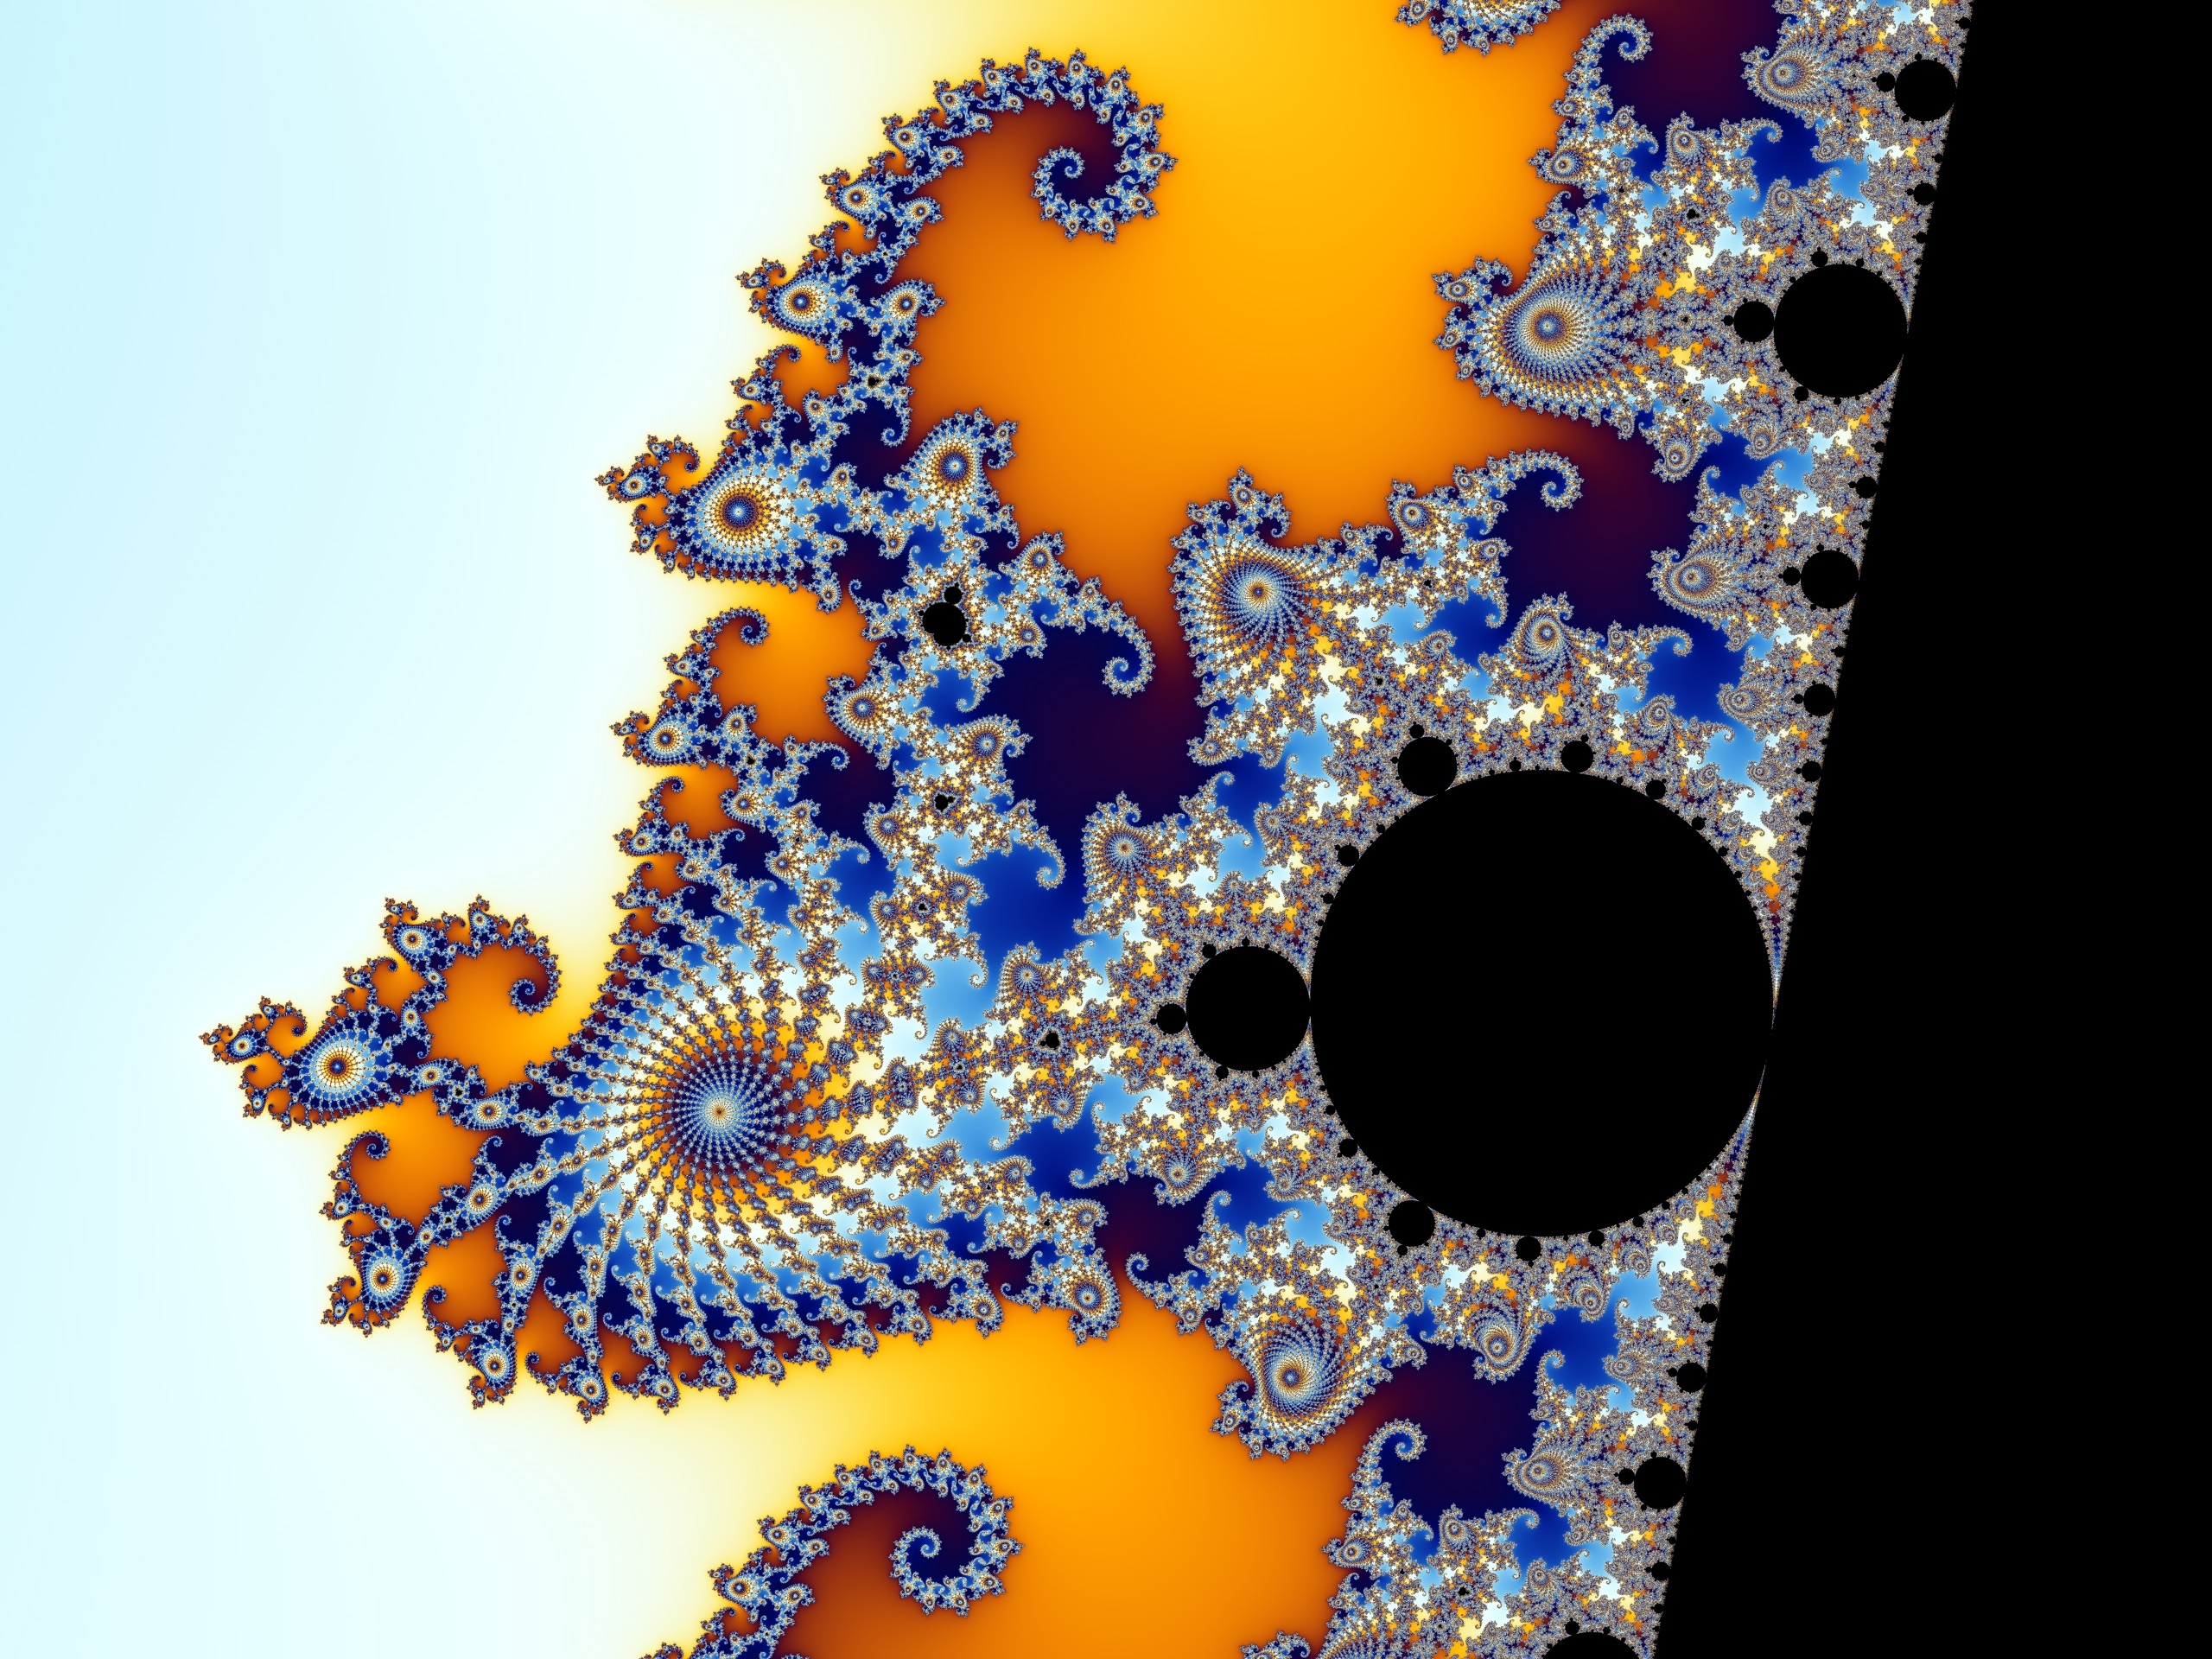
\includegraphics[width=\linewidth]{ms4.jpg}
		\caption{Seahorse}
		\label{fig:ms4}
	\end{subfigure}
	\caption{}
	\label{fig:ms}
\end{figure}
\subsubsection*{Boundaries of Periodic Orbits}
The fixed points of period one are given by
\begin{equation}
	z=z^2+c=f_c(z)\quad\rightarrow\quad z_{1,1}=\frac{1+\sqrt{1-4c}}{2}\qquad z_{1,2}=\frac{1-\sqrt{1-4c}}{2}
\end{equation}
where $z_{m,n}$ is the $n^{th}$ fixed point of period $m$.
For stability,
\begin{equation}
\frac{df_c}{dz}=2z=re^{i\theta}\quad\text{where}\quad r\geq0\quad0\leq\theta<2\pi\quad\rightarrow\quad c=\frac{re^{i\theta}}{2}-\frac{r^2e^{i2\theta}}{4}
\end{equation}
The boundary of points of period one is given by
\begin{equation}
	\left|\frac{df_c}{dz}(z_{1,1})\right|=|2z_{1,1}|=r=1
\end{equation}
\begin{equation}
	\text{Let}\ c=x+iy\quad\rightarrow\quad x=\frac{1}{2}\cos\theta-\frac{1}{4}\cos(2\theta)\qquad y=\frac{1}{2}\sin\theta-\frac{1}{4}\sin(2\theta)
\end{equation}
The parametric curve is plotted in Figure (\ref{fig:bpoms}) and forms a \textbf{cardioid} that lies at the heart of the Mandelbrot set.
\begin{wrapfigure}{r}{0.3\linewidth}
	\centering
	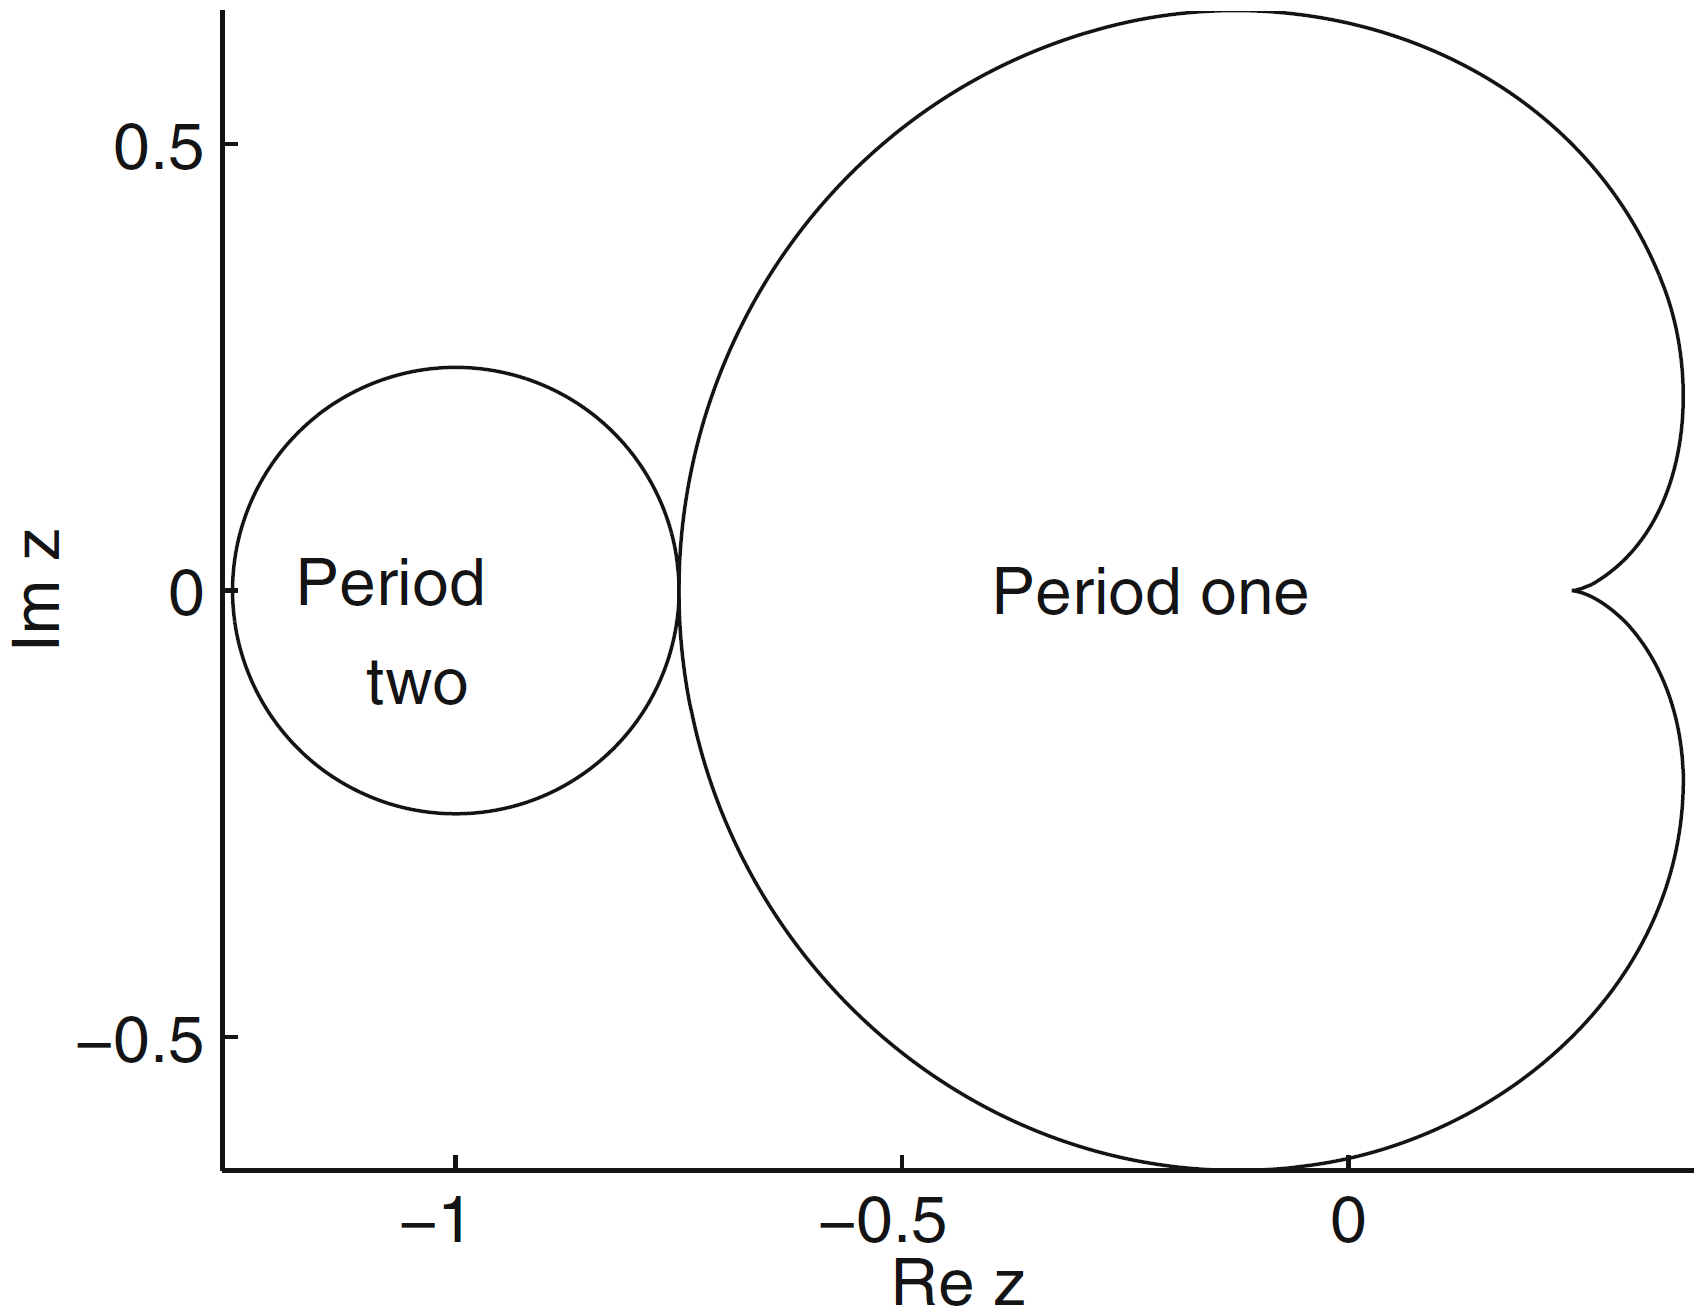
\includegraphics[width=\linewidth]{bpoms.png}
	\caption{The boundary of fixed points of periods one and two for the Mandelbrot set.}
	\label{fig:bpoms}
\end{wrapfigure}
Using similar arguments to those above, it is not difficult to extend the analysis to determine the boundary for the fixed points of period two.
\begin{equation}{\label{eq:p2ms1}}
	f_c^2(z)=(z^2+c)^2+c=z\quad\rightarrow\quad
	\begin{aligned}
		z^4+2cz^2-z+c^2+c&=0\\
		(z^2-z+c)(z^2+z+c+1)&=0
	\end{aligned}
\end{equation}
$z_{1,1}$ and $z_{1,2}$ satisfy equation (\ref{eq:p2ms1}).
\begin{equation*}
	z^2+z+c+1=0\quad\rightarrow\quad z_{2,1}=\frac{-1+\sqrt{-3-4c}}{2}\qquad z_{2,2}=\frac{-1-\sqrt{-3-4c}}{2}
\end{equation*}
The stability of each critical point is determined from the derivative of the map at the point
\begin{equation*}
	\frac{df_c^2}{dz}=4z(z^2+c)\quad\rightarrow\quad\left|\frac{df_c^2}{dz}(z_{2,1})\right|=|4+4c|\quad\text{the boundary is given by}\quad|c+1|=\frac{1}{4}
\end{equation*}
The parametric curve is plotted in Figure (\ref{fig:bpoms}) and forms a \textbf{circle} centered at $(-1,0)$ of radius $\dfrac{1}{4}$ in the Argand plane.
\subsubsection{The Newton Fractal}
The Newton-Raphson method, can be used to find the roots of the equation $f(z)=0$ using the iterative formula
\begin{equation}
	z_{n+1}=z_n-\frac{f(z_n)}{f^\prime(z_n)}
\end{equation}
\begin{figure}[H]
	\centering
	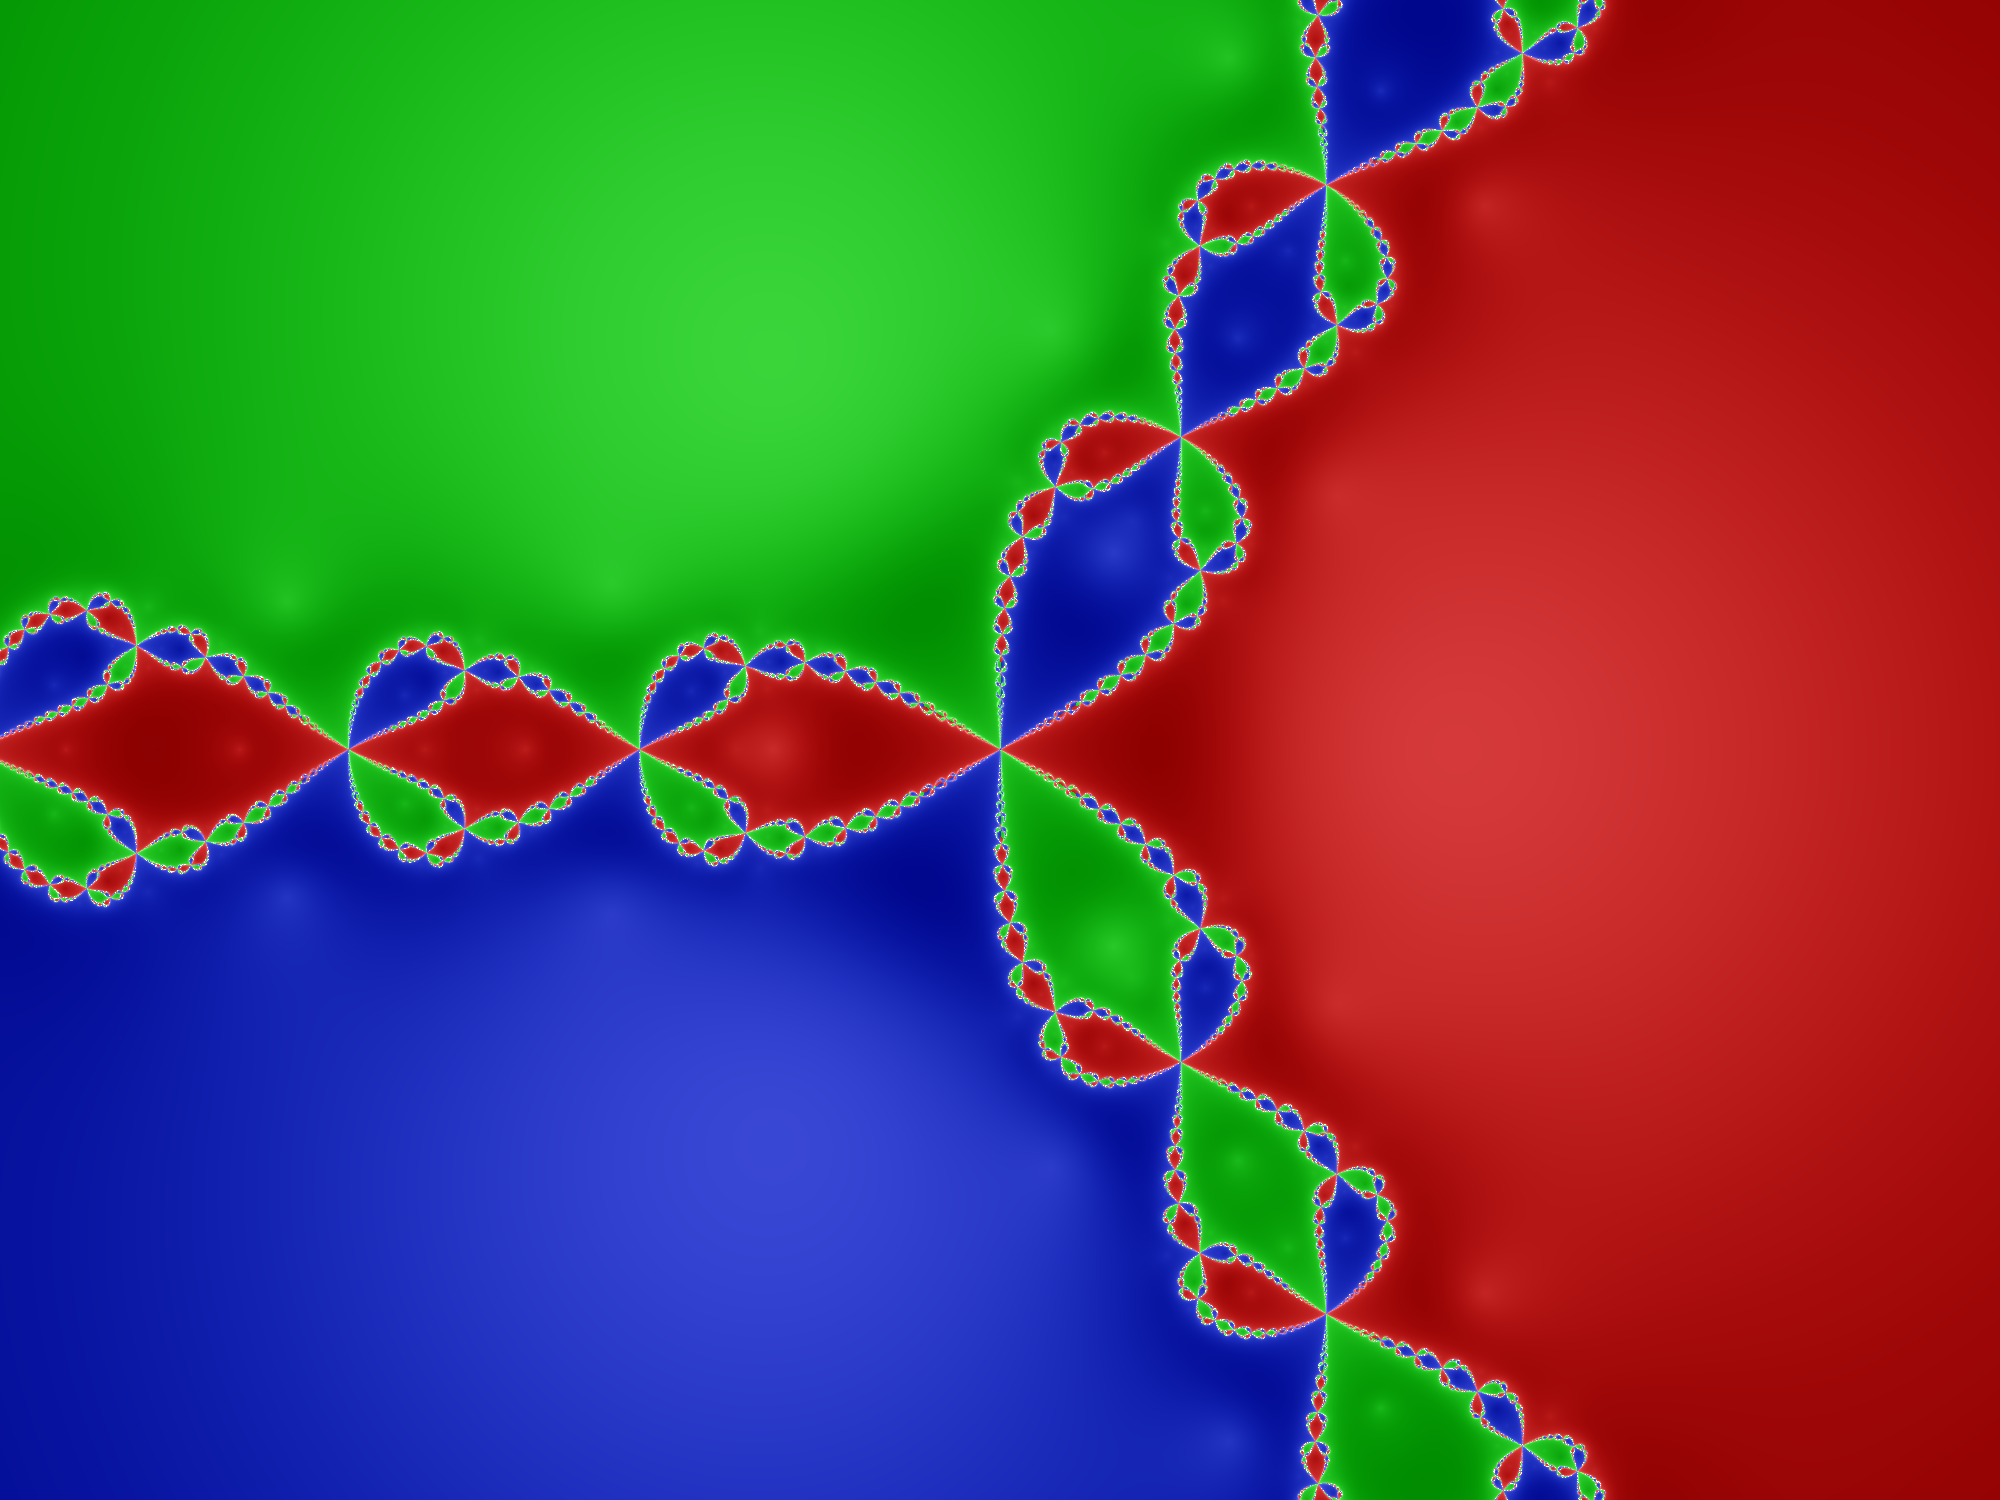
\includegraphics[width=0.6\linewidth]{nf.png}
	\caption{Julia sets for the rational function associated with Newton’s method for $f(z)=z^3-1$}
	\label{fig:nf}
\end{figure}
A Newton fractal is the Julia set of $f(z_n)$ and shows that the numerical method can be very sensitive to its choice of initial starting point.\\
In Figure (\ref{fig:nf}),
\begin{itemize}
	\item All points in the red regions are in the basin of attraction for the fixed point at $\tilde{z}_1=1$.
	\item All points in the green regions are in the basin of attraction for the fixed point at $\tilde{z}_2=\dfrac{-1+\sqrt{3}i}{2}$.
	\item And all points in the blue regions are in the basin of attraction for the fixed point at $\tilde{z}_3=\dfrac{-1-\sqrt{3}i}{2}$.
\end{itemize}
The boundary between the different basins of attraction forms a Julia set.
{\let\thefootnote\relax\footnote{{The colors in Figure (\ref{fig:ms}) are determined by the number of iterations the points take to go out of bounding region}.}}